% Options for packages loaded elsewhere
\PassOptionsToPackage{unicode}{hyperref}
\PassOptionsToPackage{hyphens}{url}
%
\documentclass[
  12pt,
]{article}
\usepackage{amsmath,amssymb}
\usepackage{lmodern}
\usepackage{iftex}
\ifPDFTeX
  \usepackage[T1]{fontenc}
  \usepackage[utf8]{inputenc}
  \usepackage{textcomp} % provide euro and other symbols
\else % if luatex or xetex
  \usepackage{unicode-math}
  \defaultfontfeatures{Scale=MatchLowercase}
  \defaultfontfeatures[\rmfamily]{Ligatures=TeX,Scale=1}
\fi
% Use upquote if available, for straight quotes in verbatim environments
\IfFileExists{upquote.sty}{\usepackage{upquote}}{}
\IfFileExists{microtype.sty}{% use microtype if available
  \usepackage[]{microtype}
  \UseMicrotypeSet[protrusion]{basicmath} % disable protrusion for tt fonts
}{}
\usepackage{xcolor}
\usepackage[margin=1in]{geometry}
\usepackage{longtable,booktabs,array}
\usepackage{calc} % for calculating minipage widths
% Correct order of tables after \paragraph or \subparagraph
\usepackage{etoolbox}
\makeatletter
\patchcmd\longtable{\par}{\if@noskipsec\mbox{}\fi\par}{}{}
\makeatother
% Allow footnotes in longtable head/foot
\IfFileExists{footnotehyper.sty}{\usepackage{footnotehyper}}{\usepackage{footnote}}
\makesavenoteenv{longtable}
\usepackage{graphicx}
\makeatletter
\def\maxwidth{\ifdim\Gin@nat@width>\linewidth\linewidth\else\Gin@nat@width\fi}
\def\maxheight{\ifdim\Gin@nat@height>\textheight\textheight\else\Gin@nat@height\fi}
\makeatother
% Scale images if necessary, so that they will not overflow the page
% margins by default, and it is still possible to overwrite the defaults
% using explicit options in \includegraphics[width, height, ...]{}
\setkeys{Gin}{width=\maxwidth,height=\maxheight,keepaspectratio}
% Set default figure placement to htbp
\makeatletter
\def\fps@figure{htbp}
\makeatother
\setlength{\emergencystretch}{3em} % prevent overfull lines
\providecommand{\tightlist}{%
  \setlength{\itemsep}{0pt}\setlength{\parskip}{0pt}}
\setcounter{secnumdepth}{5}
\newlength{\cslhangindent}
\setlength{\cslhangindent}{1.5em}
\newlength{\csllabelwidth}
\setlength{\csllabelwidth}{3em}
\newlength{\cslentryspacingunit} % times entry-spacing
\setlength{\cslentryspacingunit}{\parskip}
\newenvironment{CSLReferences}[2] % #1 hanging-ident, #2 entry spacing
 {% don't indent paragraphs
  \setlength{\parindent}{0pt}
  % turn on hanging indent if param 1 is 1
  \ifodd #1
  \let\oldpar\par
  \def\par{\hangindent=\cslhangindent\oldpar}
  \fi
  % set entry spacing
  \setlength{\parskip}{#2\cslentryspacingunit}
 }%
 {}
\usepackage{calc}
\newcommand{\CSLBlock}[1]{#1\hfill\break}
\newcommand{\CSLLeftMargin}[1]{\parbox[t]{\csllabelwidth}{#1}}
\newcommand{\CSLRightInline}[1]{\parbox[t]{\linewidth - \csllabelwidth}{#1}\break}
\newcommand{\CSLIndent}[1]{\hspace{\cslhangindent}#1}
\usepackage{mathptmx} %to use times new roman font
\usepackage[flushleft]{threeparttable}
\usepackage{multirow}
\usepackage{multicol}
\usepackage{booktabs,caption}
\usepackage{pdflscape}
\usepackage{indentfirst}
\usepackage{float}
\usepackage{longtable}
\usepackage{array}
\usepackage{wrapfig}
\usepackage{float}
\usepackage{colortbl}
\usepackage{tabu}
\usepackage{threeparttablex}
\usepackage[normalem]{ulem}
\usepackage{makecell}
\usepackage{xcolor}
\usepackage{siunitx}
\sisetup{round-mode = places, round-precision = 4,}
\interfootnotelinepenalty=10000
\usepackage{setspace}
  \doublespacing
\usepackage{booktabs}
\usepackage{longtable}
\usepackage{array}
\usepackage{multirow}
\usepackage{wrapfig}
\usepackage{float}
\usepackage{colortbl}
\usepackage{pdflscape}
\usepackage{tabu}
\usepackage{threeparttable}
\usepackage{threeparttablex}
\usepackage[normalem]{ulem}
\usepackage{makecell}
\usepackage{xcolor}
\ifLuaTeX
  \usepackage{selnolig}  % disable illegal ligatures
\fi
\IfFileExists{bookmark.sty}{\usepackage{bookmark}}{\usepackage{hyperref}}
\IfFileExists{xurl.sty}{\usepackage{xurl}}{} % add URL line breaks if available
\urlstyle{same} % disable monospaced font for URLs
\hypersetup{
  pdftitle={Identify Unsustainable Credit Gap},
  pdfauthor={Nam Nguyen},
  hidelinks,
  pdfcreator={LaTeX via pandoc}}

\title{Identify Unsustainable Credit Gap}
\author{Nam Nguyen}
\date{July 28, 2022}

\begin{document}
\maketitle
\begin{abstract}
To overcome model uncertainty in using credit gap as an early warning indicator (EWI) of systemic financial crises in a binary outcome setting, we propose using model averaging of different credit gap measurements to achieve a better averaged model fit and out-of-sample prediction. The methodology we use is logistic binary regression in a panel setup consisting of 40 countries. In this paper, we also propose a novel, superior criteria to judge the performance of an EWI than the one currently popularly used in the literature. Additionally, the empirical results showed that our Bayesian averaged model could synthesize a single credit gap that outperforms any other popularly studied credit gap measurements in terms of an early warning indicator.
\end{abstract}

\hypertarget{introduction}{%
\section{Introduction}\label{introduction}}

Credit-to-GDP gaps have been identified as the top candidate as an early warning indicator (EWI) for future financial crises. As the importance of the financial market to the real economy has increased, failing to predict a future systemic crisis and missing the correct timing to implement macroprudential instruments such as Countercyclical Capital Buffer (CCyB) can lead to significant economic losses. As a result, there is a need to improve the performance of our early warning indicator model, specifically when using the credit gap in univariate EWI models.

In the EWI literature, The Bank of International Settlement (BIS) Basel credit gap using a real-time (one-sided) version of the Hodrick-Prescott filter (HP) has been established as a reference point for policymakers. The BIS Basel gap is easy to implement and communicate; traditionally, it has performed well as an early indicator. However, recent literature has found evidence that optimizing parameters of various decomposition filters can improve those filters' performance beyond the predictive power of the BIS Basel gap as an EWI. The details are discussed in Drehmann \& Yetman (\protect\hyperlink{ref-drehmann_which_2021}{2021}) and Beltran, Jahan-Parvar, \& Paine (\protect\hyperlink{ref-beltran_optimizing_2021}{2021}).

The development of embedding optimization of decomposition filter into the process of building an EWI framework has significantly improved the performance of the credit gap filters. However, this also created another issue which is model uncertainty. Policymakers now face at least five decomposition methods, each with different feature parameters to consider optimizing for, such as smoothing parameters, robustness, and rolling window. Furthermore, changes in the sample window would change the performance of those filters with optimized parameters. Selecting a robust and best-performing decomposition filter and optimizing its feature parameters can be a paradox of choice for policymakers.

There is a need for a robust methodology to create a univariate EWI that adapts well to changes in dynamics of the underlying financial market but at the same time uses only the credit gap as an explanatory variable. This paper attempts to solve the model uncertainty issue by using Bayesian model selection and average methods. We first create a set of possible decomposition filters with rich features from the recent literature findings. Out of all possible initial credit gaps created, We then implement a series of model selection and discarding using an additional novel metric psAUC (partial standardized area under the curve of receiver operating characteristic), discussed in subsection \ref{psAUC}. Subsequently, from a finalized subset of variables that passed the performance filters, we perform model averaging of all possible combinations of the variables. Raftery (\protect\hyperlink{ref-raftery_bayesian_1995}{1995}) proposed the Bayesian model average method that averages its estimated parameters of interest across all possible combinations of variables. The model that uses the average estimate has proven to be more robust and performs better in out-of-sample forecasts than any other individual model in the selected subset of model combinations.

Using data from 1970:Q4 to 2017:Q4 across 43 countries, we created 90 credit gaps with varying features found in the literature. We implemented the model selection and average methods described in the paragraph above. We then found evidence that the new EWI performance metric partially standarized AUC (psAUC), which constraints analysis to the region where Type II error \textless{} 1/3, to be a robust single value criterion. We also successfully incorporated the new metric into our model selection and averaging method. Lastly, to ease policy implications, we propose to create a single credit gap measurement from weighted-averaging other popularly studied credit gap measurements. The single weighted average credit gap is tested as more robust in resampling bootstrapping estimates. It performs better in out-of-sample forecasts k-fold cross-validation than any other individual model in the filtered subset of model combinations.

The paper is structured as follows. In the next section, we discuss relevant branches of literature. In Section 3, we describe the data used in this paper. Section 4 outlines the methodology I use for model selection, model average, and a weighted combination of variables of interest, as well as a novel metric for testing the performance of the selected variable and averaged model. Section 5 describes the empirical results of the selected variables in the horse race. Section 6 analyzes time series graphs of individual countries. Section 7 summarizes the main conclusions.

\hypertarget{literature-review}{%
\section{Literature Review}\label{literature-review}}

In this section, we discuss the branches of literature that our study is relevant and contributes to.

C. Borio \& Lowe (\protect\hyperlink{ref-borio_assessing_2002}{2002}) first documented credit gaps' property as a useful early warning indicator (EWI) for banking crises. Earlier literature on excessive credit leading to crises includes Minsky (\protect\hyperlink{ref-minsky_financial_1977}{1977}), Manias (\protect\hyperlink{ref-manias_panics_1978}{1978}), and Kaminsky \& Reinhart (\protect\hyperlink{ref-kaminsky_twin_1999}{1999}).

C. E. V. Borio \& Drehmann (\protect\hyperlink{ref-borio_assessing_2009}{2009}) assessed different smoothing parameters for the one-sided HP filter and later determined \(\lambda=400,000\) to be the ideal value for measuring credit gap based on its long smooth trend property and performance as an early warning indicator. Banking Supervision (2010) (\protect\hyperlink{ref-basel_guidance_2010}{2010}) later established this particular HP filter as the Basel credit gap (we call it BIS Basel gap in this paper), and it became the reference for all EWI models using credit gap filters. Drehmann \& Tsatsaronis (\protect\hyperlink{ref-drehmann_credit_2014}{2014}) defended the Basel gap's performance as an EWI against criticism it received, such as its failure to perform well in emerging market economies.

Drehmann \& Juselius (\protect\hyperlink{ref-drehmann_evaluating_2014}{2014}) set out a list of criteria for an EWI. It needs to have the ``right timing'' of being able to detect future financial crises from 20-6 quarters ahead of a future systemic crisis; a ``stable signal'' that does not decrease as the periods approach the actual crises date; ``robustness'' that fits well with different data set; and ``interpretability'' which is ideal for a univariate model such as the credit gap to determine an optimized threshold of classifying excessive credit. Lastly, EWI \(S_i\) outperforms EWI \(S_j\) for horizon h if \(AUC(S_{i,h}) > AUC(S_{j,h})\). This last criterion, however, receives criticism regarding the lower left region of the ROC curve that represents low predictive power of a model, which the AUC metric also measures.\footnote{the details are discussed in subsection \ref{psAUC}}

C. Borio (\protect\hyperlink{ref-borio_financial_2014}{2014}) established that credit cycles have a much lower frequency than business cycles. It also pointed out that credit cycle peaks are closely associated with the onset of financial crises. Because of that property, they can detect crises in real-time within macroprudential policies implementation window.

Hamilton (\protect\hyperlink{ref-hamilton_why_2018}{2018}) argues against using HP filter for macroeconomics series as it introduces spurious dynamics. Drehmann \& Yetman (\protect\hyperlink{ref-drehmann_why_2018}{2018}) defended the HP filter again but will later admit other filters with additional features, such as a Hamilton filter estimated in a panel setting, outperformed the Basel gap in Drehmann \& Yetman (\protect\hyperlink{ref-drehmann_which_2021}{2021}).

Additionally, features for the decomposition methods include rolling sample windows of 15 and 20 years as proposed by Galán (\protect\hyperlink{ref-galan_measuring_2019}{2019}) to help improve the performance of the decomposition filter. Beltran et al. (\protect\hyperlink{ref-beltran_optimizing_2021}{2021}) embedded the optimization of features parameters into the construction of an EWI model and constraint the search range for the loss function to the region where True Positive rates \(\ge\) 2/3 or Type II error rates \textless{} 2/3 following suggestions in C. E. V. Borio \& Drehmann (\protect\hyperlink{ref-borio_assessing_2009}{2009}), the paper also introduced using Structural Time Series model (STM) gap, Moving average (MA) gap as possible candidates for the EWI model.

Galán (\protect\hyperlink{ref-galan_measuring_2019}{2019}) also proposed adding other features to the Basel gap that individual countries implement that are out of the scope of this paper's implementation. Such adjustments include adjusting for GDP decrease, combining one and two-sided filters for robustness, adjusting by projection as in Gerdrup, Kvinlog, \& Schaanning (\protect\hyperlink{ref-gerdrup_key_2013}{2013}), and adjusting for currency fluctuations.

However, there is no consensus on which decomposition with which features would be the best performing and most robust EWI. In this paper, we aim to construct a methodology to find the best combination of decomposition and features to be used as an EWI and propose an average model that performs as well as the best combination, if not better. The methodology we use for the model selection, and average steps are discussed in the literature branch below.

Babecký et al. (\protect\hyperlink{ref-babecky_banking_2014}{2014}) used a model selection method called Markov Chain Monte Carlo Model Comparison (\(MC^3\)) developed by Madigan, York, \& Allard (\protect\hyperlink{ref-madigan_bayesian_1995}{1995}). This method allows for a feasible search for best-fitted combinations out of a large set of variables with similar features, which would not be correctly estimated using other model selection methods such as RIDGE, LASSO, and Elastic Net. Furnival \& Wilson (\protect\hyperlink{ref-furnival_regressions_2000}{2000}) proposed a ``leap and bound'' algorithm to find the best-fitted subsets without examining all possible subsets of variables.

The Bayesian model averaging method is formally described in Raftery (\protect\hyperlink{ref-raftery_bayesian_1995}{1995}). It aims to overcome model uncertainty by averaging the performance of a set of models. The averaged model performs better than the individual models on out-of-sample forecasts. Recently, Holopainen \& Sarlin (\protect\hyperlink{ref-holopainen_toward_2017}{2017}) implemented ensemble methods to combine various machine learning model predictions and found significant improvement in the model performance.

The model average method could be applied to a multivariate setting, but that will cost us the ability to synthesize a combined weighted credit gap. Following the motivation from Chapter 3, we also attempt to create a combined weighted credit gap in this chapter that performs well in a horse race with other credit gap measurements.

Multivariate early warning system (EWS) is also a significant branch of early warning literature and is worth mentioning. The variables selected in Babecký et al. (\protect\hyperlink{ref-babecky_banking_2014}{2014}) that perform well in EWS are then used in the following papers. Drehmann \& Juselius (\protect\hyperlink{ref-drehmann_evaluating_2014}{2014}) established that with the credit gap, the Debt-to-Service ratio is another EWI that performs well within 1-4 quarters of the future systemic financial crisis. Aldasoro, Borio, \& Drehmann (\protect\hyperlink{ref-aldasoro_early_2018}{2018}) is an extension of Drehmann \& Juselius (\protect\hyperlink{ref-drehmann_evaluating_2014}{2014}). Furthermore, Alessi \& Detken (\protect\hyperlink{ref-alessi_identifying_2018}{2018}) used a Random Forest model to achieve a higher EWI performance metric than traditional generalized linear regression. Even though multivariate models can achieve higher model fit and prediction accuracy than univariate models, they also require richer data availability and limit the scope of the model implementation. Certain Emerging market economies with insufficient data would benefit more from a well-performing univariate model.

Lastly, we touch on the literature on partial estimating the Area Under the Curve of Receiver Operating Characteristic (psAUC). Detken et al. (\protect\hyperlink{ref-detken_operationalising_2014}{2014}) first introduced the use of partial standardized AUC in the EWI setting. The partial standardized AUC is popularly studied in the medical statistics literature, e.g., McClish (\protect\hyperlink{ref-mcclish_analyzing_1989}{1989}), but is relatively new in the EWI literature. We will use this novel (psAUC) metric, inspired by both Detken et al. (\protect\hyperlink{ref-detken_operationalising_2014}{2014}) and the policy function restriction in Beltran et al. (\protect\hyperlink{ref-beltran_optimizing_2021}{2021}), to improve our model selection and averaging process in terms of satisfying policy implication requirements (e.g.~TPR \(\ge\) 2/3). The method for partial estimation of the ROC curve is documented in Robin et al. (\protect\hyperlink{ref-robin_proc_2011}{2011}).

\hypertarget{data-description}{%
\section{Data Description}\label{data-description}}

Our sample periods include quarterly data from 1970:Q4 to 2017:Q4 across 43 countries.\footnote{The list of countries with data available are: Argentina, Austria, Australia, Belgium, Brazil, Canada, Switzerland, Chile, China, Colombia, Czech Republic, Germany, Denmark, Spain, Finland, France, United Kingdom, Greece, Hong Kong SAR, Hungary, Indonesia, Ireland, Israel, India, Italy, Japan, Korea, Luxembourg, Mexico, Malaysia, Netherlands, Norway, New Zealand, Poland, Portugal, Russia, Saudi Arabia, Sweden, Singapore, Thailand, Turkey, United States, South Africa} The sample periods were chosen based on the availability of systemic crisis data and total credit to GDP ratio data. The primary source of the data comes from the Bank of International Settlement (BIS). The credit data is measured as total credit to the private non-financial sector as a percentage of GDP.\footnote{Source of the data could be accessed here: \url{https://www.bis.org/statistics/totcredit/credpriv_doc.pdf}}

Regarding data for dating systemic crises, there is no single consensus source of database. We follow the literature and use the crisis dates reported in the European Systemic Risk Board crisis data set (Lo Duca et al.~2017) and Laeven and Valencia (2018), which include systemic crisis data from after WWII. However, the first systemic crisis did not happen until the early 1970s.

There are three types of crises: banking, currency, and debt crises, all of which could lead to a systemic crisis. A crisis can be labeled as systemic when certain conditions are met, such as significant signs of financial distress in the banking system, bank runs, and significant policy intervention measurements are imposed. The authors also consulted with subject matter experts in each country to determine the dates of details of the systemic crises.

While the credit data is available until 2021:Q3, our systemic crisis data stopped at 2017:Q4. Therefore, we will limit our analysis till 2017:Q4. We will also omit periods of countries with shorter measurements of credit.

\hypertarget{model}{%
\section{Empirical Methodology}\label{model}}

\hypertarget{overview}{%
\subsection{Overview}\label{overview}}

The total credit series is nonstationary. In order to extract a useful stationary credit signal to use as an early warning indicator for future financial crises, we first decompose the series into a nonstationary trend and a stationary cycle using various popularly studied filters in subsection \ref{decomp}.

The idea behind using the credit gap as an early warning indicator is that a prolonged period of excessive credit growth could be linked to future financial crises. Therefore, we can use logistic regression to identify pre-crisis periods with unsustainable high credit gap values over a certain threshold.

In subsection \ref{logistic-regression}, we discuss strategies for identifying the dependent variable (pre-crisis periods) and the logistic regression empirical method. In subsection \ref{metrics} we then discuss the metrics to determine the performance of a credit gap as an early warning indicator EWI model such as BIC, AIC values, Area Under Curve (AUC) of receiver operating characteristic, how we determine a policy loss function, optimize credit gap threshold and estimate the minimized Type I and Type II error rates. We will then propose a novel metric - partial standardized AUC (psAUC) that, when used in conjunction with other metrics, will provide more desirable properties in terms of policy implication and overcome some of the criticism that the traditional AUC metric receives.

This paper aims to overcome model uncertainty when using credit gap filters as an early warning indicator for future financial crises. Since each decomposition filter of the total credit series provides a stationary series that performs qualitatively differently from other filters as an EWI, we propose selecting the best gap candidates and performing model averaging to achieve model stability and improved out-of-sample prediction as proposed in (\protect\hyperlink{ref-raftery_bayesian_1995}{Raftery, 1995}).

In subsection \ref{modelselection}, we will use the metrics discussed in subsection \ref{logistic-regression} to select credit gap filters that perform well individually and in combination with other credit gaps. Then in subsection \ref{model-average}, we discuss the theory behind the Bayesian model average method, our model customization to fit our need, and the new metric (psAUC).

Lastly, in subsection \ref{weighted-gap-creation}, for ease of policy implication, we propose the creation of a crisis-weighted credit gap that would inherit the information and features from the averaged model of 30 other credit gaps, and would perform as well as the averaged model prediction does.

\hypertarget{decomp}{%
\subsection{Credit gap decompositions}\label{decomp}}

\begin{align}
    100*\frac{Credit}{GDP} &= y_it = \tau_{itj} + c_{itj}
\end{align}

We started our variable selection process by creating 90 candidate one-sided credit gap measurements based on the literature.\footnote{List of filters created is can be viewed in Appendix \ref{filterslist}} The nonstationary Credit to GDP ratio series is decomposed into a nonstationary trend \(\tau_{yit}\) and a stationary cycle credit gap \(c_{itj}\) components. Once a country has more than 15 years of credit measurement available, we start storing its one-sided credit gap values onward. Our decomposition filter methods include one-sided Hodrick-Prescott, Hamilton (panel and non-panel setting), Moving Average, Structural Time-series model, Beveridge-Nelson, linear, quadratic, and polynomial decompositions. All are decomposed with full sample, rolling 15 years and 20 years rolling window feature when possible.

Apart from the filters that we already introduced in Chapter 3 - ``Measuring credit gap'' (Equations 3.1 - 3.5), the two additional filters we will use in this chapter are Moving Average, Structural Time-Series model filters that Beltran et al. (\protect\hyperlink{ref-beltran_optimizing_2021}{2021}) introduced.\footnote{Refer to their equation representations here in Appendix \ref{ma-stm-eq}}

\hypertarget{logistic-regression}{%
\subsection{Early Warning Indicator - GLM Logistic regression}\label{logistic-regression}}

We begin testing the fitness of the EWI model using credit gap measurements by implementing binary logistic regression. We identify our dependent variable as the periods of 5-12 quarters ahead of a systemic financial crisis. The underlying classification model assumes that the credit to GDP ratio gap will increase sharply as a response to an excessive credit increase due to expansionary monetary policy or a sharp decline in GDP, which is the ratio's denominator. When the credit gap is above a certain threshold for a prolonged period, it signals that the economy is at risk of a future financial crisis. The periods with excessive credit before financial crises will be labeled pre-crisis periods.

It is also worth pointing out that there is no consensus on setting the periods to label as pre-crisis. The literature labeled pre-crisis periods with various ranges from 1-16 quarters before a crisis. We decided to use a labeling strategy with ideal policy implication properties. It is recommended that macroprudential policy takes more than four quarters to be effective because of policy implementation lag. As a result, a signal telling that the economy will experience a financial crisis in 1-4 quarters has little policy implication. Therefore, we start labeling the pre-crisis periods in the 5th quarter before a systemic crisis. We stop labeling in the 12th quarter before a crisis because implementing counter-cyclical policy too early will be ineffective in lowering the risk of a future crisis and would only exacerbate economic conditions by unnecessary credit tightening.

Equation \eqref{eq:logit} represents the binary logistic regression:

\begin{align} \label{eq:logit}
  pre.crisis_{it} \sim c_{itj} 
\end{align}

In which \(i\) is the country indicator, and \(j\) is the credit gap filter type. The binary dependent variable \(pre.crisis_{it}\) takes values of 1 when the economy is between 5-12 quarters before a systemic financial crisis labeling the periods as ``pre-crisis'' positive. We discard measurements between 1-4 quarters before a crisis, during, and post-crisis management periods identified in Lo Duca et al.~(2017) and Laeven and Valencia (2018). The measurements in these periods are discarded to avoid biased estimation as credit gaps behave erratically during a crisis.

The indicator is set to 0 at other periods. Additionally, pre-crisis periods of imported crises identified in the dataset are set to 0 since the model aims to capture pre-crisis periods created by a country's excess credit growth, not from exogenous shocks. However, for labeling conformity, we still discard measurements of periods during and post-crisis of these imported crises, as countries experiencing imported crises could implement reactionary monetary policies.

\hypertarget{metrics}{%
\subsection{EWI performance metrics}\label{metrics}}

\hypertarget{likelihood-values-and-bic}{%
\subsubsection{Likelihood values and BIC}\label{likelihood-values-and-bic}}

The logistic regression model parameters are estimated by maximizing the cross-entropy log-likelihood values. The relationship between the BIC (Bayesian Information Criterion) and likelihood value is expressed in Equation \eqref{eq:BIC-lik}. The model selection criterion here is to choose the filter method with a lower BIC value associated with a higher likelihood value and fitness of the general linearized model or a higher degree of freedom by using fewer explanatory variables.

\hypertarget{area-under-the-curve-auc-of-receiver-operating-characteristic-roc}{%
\subsubsection{Area Under the Curve (AUC) of receiver operating characteristic (ROC)}\label{area-under-the-curve-auc-of-receiver-operating-characteristic-roc}}

A receiver operating characteristic (ROC) curve in the EWI literature setting represents True Positive Rate (TPR) and False Positive Rate (FPR) Cartesian coordinates of different credit gap thresholds, which are used as indicators for identifying pre-crisis periods.\footnote{Refer to Figure \ref{fig:psAUCfig} for illustration} The credit gap thresholds are determined by the logistic regression model predicted response values which range from (0,1) and map increasingly with the credit gap magnitude values.

A logistic model is strictly preferred over another comparable model if all of the coordinates of its ROC curve are closer to the top-left region of the graph, which minimizes FPR and maximizes TPR. However, that is not always the case when we have such a clear-cut difference. Models can have overlapping ROC curves. To simplify the process of model selection in such cases, the area under the curve (AUC) of ROC metric is used.

\begin{align*}
AUC = \int_0^1 TPR d(FPR)
\end{align*}

Each logistic regression with a different gap measurement yields an Area Under Curve (AUC) of receiver operating characteristic value. There is an underlying assumption that the higher the AUC value is, the better the overall performance of a credit gap is as an EWI since, on average, its ROC curve has coordinates with higher TPR and lower FPR.

True Positive Rate represents a model's predictive power (P) to identify pre-crisis periods correctly (positive case). \(TPR = TP / (TP + FN)\). False Positive Rate represents the Type I error rate that a model misidentifies a calm, normal period (negative case) as a pre-crisis period (positive case). \(FPR = FP / (FP + TN)\). Lastly, we discuss the False Negative Rate or the Type II error rate at which a model misidentifies a pre-crisis period (positive case) as a normal calm period (negative case). \(FNR = 1 - TPR = FN / (TP + FN)\).\footnote{Our notation of Type I and Type II error follows Beltran (2021) which deviated from previous literature.}

Central planners working with classification problems have dual objectives to minimize Type I and Type II errors. To simplify this problem, a policy loss function with the input of the two error types are used:

\begin{align} \label{eq:policylossold}
L_{\theta,\rho}=\alpha TypeI(\theta)+(1-\alpha)TypeII(\theta)
\end{align}

With \(\alpha = 0.5\) by default if policymakers are indifferent about the two types of errors. Here, the model selection criteria would be to select minimized policy loss function with the smallest combination of Type I and Type II error rates.

A binary logistic regression model with a substantially higher AUC value will have smaller sets of Type I and Type II metrics values. Therefore, its optimized credit gap threshold value that minimizes the policy loss function would represent superior Type I and Type II error rates.

However, because the AUC value is an aggregate value representing information of the whole ROC curve, the area on its lower left corner, where the predictive power of the threshold (TPR) is low, and type II error rates are high, is not relevant for policy implications discussion. Before the Great Financial Crisis of 2008, central planners tended to weigh Type I errors more than Type II errors since the cost of misspecifying a financial crisis was not apparent, and a Type I error meant costing the economy unnecessary credit constraints by implementing reactionary policies. However, since 2009, there has been a shift in weighing Type II errors more as the cost of misspecifying a systemic financial crisis became significantly heavier than a Type I error.

\hypertarget{psAUC}{%
\subsubsection{Partial standardised AUC}\label{psAUC}}

To overcome the issue of unnecessary information included in the full AUC. An approach to estimate only a partial relevant area under the ROC was proposed in McClish (\protect\hyperlink{ref-mcclish_analyzing_1989}{1989}) and later implemented in the EWI setting by Detken et al. (\protect\hyperlink{ref-detken_operationalising_2014}{2014}). We will also discuss the standardization of the partial AUC metric (psAUC) in Equation \eqref{eq:psAUCeq}.

Detken (2014) on partial standardized AUC:

\begin{quote}
``Instead of considering only the full AUROC (e.g.~Drehmann and Juselius, 2014), this paper also presents a partial standardized AUROC (psAUROC) that cuts off the area associated with a preference parameter of \(\theta<0.5\).''\ldots{}
\end{quote}

\begin{quote}
``While the psAUROC has been used extensively in the area of medical statistics to assess the performance of a classifier only in specific regions of the ROC curve (e.g., McClish, 1989 and Jiang et al., 1996), it is a new approach in the literature evaluating EWMs''\ldots{}
\end{quote}

\begin{quote}
``The results reported in this paper show that the psAUROC can reveal useful additional information as long as the partial area does not become too restricted.''
\end{quote}

Detken et al. (\protect\hyperlink{ref-detken_operationalising_2014}{2014}) proposed cutting off the area representing the preference response parameter in a multivariate regression setting. However, this application does not directly translate to a univariate credit gap model. More relevantly, (\protect\hyperlink{ref-beltran_optimizing_2021}{Beltran et al., 2021}) constrained the policy loss function to regions where TPR \(\ge 2/3\) or Type II error rate \(< 1/3\). They then estimated the policy loss function value at different points on the partial ROC curve by assigning different policy preference parameter values \(\alpha\).

To merge these two ideas above and to solve the uncertainty issue of having to estimate policy loss function at different policy preference parameter values to determine model performance, we propose to restrict the consideration of the ROC curve to TPR \(\ge 2/3\), then estimate the partial standardize psAUC of the restricted ROC curve region instead. Note in Equation \eqref{eq:pAUC}. We estimated the partial area under to curve that represents TPR and TNR (instead of TPR and FNR) and took integral along the TPR axis.

\begin{align} \label{eq:pAUC}
pAUC = \int_{\frac{2}{3}}^1 TNR \, d(TPR) = \int_{\frac{2}{3}}^1 specificity \, d(sensitivity)
\end{align}

Because we are limiting our analysis only to the portion of the ROC curve that satisfies TPR \(\ge 2/3\), the policy loss function \eqref{eq:policylossold} used in previous literature tends to have a corner solution of optimized thresholds where TPR = 2/3. We propose using an alternative policy loss function that priorities points on the ROC closest to the top left regions where both Type I and II errors are the lowest:

\begin{align*}
L_{\theta,\rho}= TypeI(\theta)^2 + TypeII(\theta)^2 = (1 - sensitivity)^2 + (1 - specificity)^2
\end{align*}

The last step is to standardize the partial AUC value:

\begin{figure}

{\centering 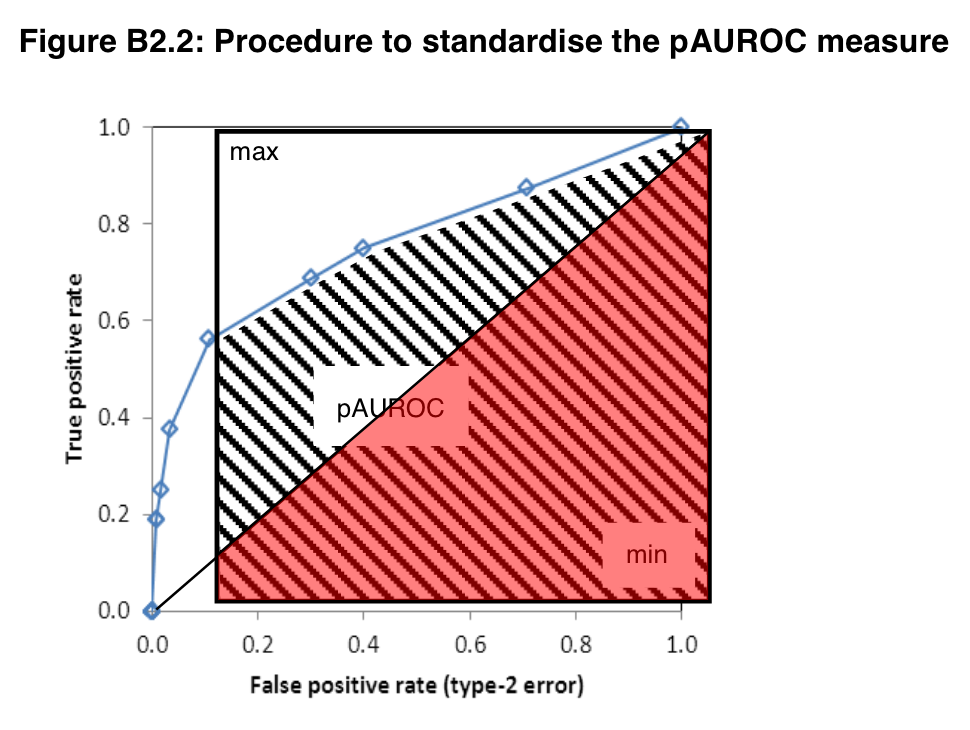
\includegraphics[width=0.7\linewidth]{../metadata/pAUC} 

}

\caption{Standardize partial AUC}\label{fig:psAUCfig}
\end{figure}

\begin{align} \label{eq:psAUCeq}
psAUC = \frac{1}{2}\left[ 1+ \frac{pAUC - min}{max - min}\right]
\end{align}

The standardization step helps with the comparison of EWI models' performance. Traditional AUC values range from 0 to 1, with 0.5 being the value for a null hypothesis model or an informationless guess. When only estimated partially, the partial AUC value will not retain the same range making it harder to interpret their meaning. Standardizing the partial AUC values restores the ranges of possible values to 0 and 1.

In section \ref{empirical-results}, we will discuss the relevance and performance of the psAUC as an EWI metric and the other metrics introduced in this subsection.

\hypertarget{modelselection}{%
\subsection{Variable Selection}\label{modelselection}}

Our overall methodology goal is to implement model averaging of top candidate variables. In order to achieve that, we need to select top EWI candidates using the EWI performance criteria discussed in the previous section. We also search for models with combinations of variables that, when combined using positive weights, would have a better model fit than a univariate model would. We aim to select 29 credit gap measurements based on these two criteria.

Firstly, we compared performances of individual credit gaps using partial area under the curve (psAUC) values. Table \ref{tab:varselect} ranked decomposition filters by psAUC.

\begin{table}[H]

\caption{\label{tab:varselect}Top 30 credit gap measurements ranked by psAUC}
\centering
\resizebox{\linewidth}{!}{
\begin{tabular}[t]{lrrr>{}rrrrr}
\toprule
Cycles & BIC & AIC & AUC & psAUC & c.Threshold & Type.I & Type.II & Policy.Loss.Function\\
\midrule
\cellcolor{gray!6}{null} & \cellcolor{gray!6}{0.0000} & \cellcolor{gray!6}{0.0000} & \cellcolor{gray!6}{0.5000} & \textbf{\cellcolor{gray!6}{0.5000}} & \cellcolor{gray!6}{} & \cellcolor{gray!6}{1.0000} & \cellcolor{gray!6}{0.0000} & \cellcolor{gray!6}{1.0000}\\
c.bn6.r20 & -108.0679 & -114.4506 & 0.7048 & \textbf{0.6379} & 0.6581 & 0.3962 & 0.3019 & 0.2481\\
\cellcolor{gray!6}{c.hamilton28.panel} & \cellcolor{gray!6}{-149.8518} & \cellcolor{gray!6}{-156.2346} & \cellcolor{gray!6}{0.7107} & \textbf{\cellcolor{gray!6}{0.6359}} & \cellcolor{gray!6}{9.7674} & \cellcolor{gray!6}{0.3912} & \cellcolor{gray!6}{0.3066} & \cellcolor{gray!6}{0.2470}\\
c.hamilton13.panelr20 & -150.2442 & -156.6269 & 0.7036 & \textbf{0.6333} & 5.9895 & 0.4261 & 0.2547 & 0.2464\\
\cellcolor{gray!6}{c.hamilton24.panel} & \cellcolor{gray!6}{-134.4093} & \cellcolor{gray!6}{-140.7920} & \cellcolor{gray!6}{0.6991} & \textbf{\cellcolor{gray!6}{0.6322}} & \cellcolor{gray!6}{7.1794} & \cellcolor{gray!6}{0.4383} & \cellcolor{gray!6}{0.2689} & \cellcolor{gray!6}{0.2644}\\
\addlinespace
c.hamilton20.panelr20 & -151.5617 & -157.9445 & 0.7048 & \textbf{0.6313} & 7.9350 & 0.4321 & 0.3066 & 0.2807\\
\cellcolor{gray!6}{c.ma} & \cellcolor{gray!6}{-120.8108} & \cellcolor{gray!6}{-127.1936} & \cellcolor{gray!6}{0.6922} & \textbf{\cellcolor{gray!6}{0.6313}} & \cellcolor{gray!6}{5.7813} & \cellcolor{gray!6}{0.3989} & \cellcolor{gray!6}{0.3160} & \cellcolor{gray!6}{0.2590}\\
c.hamilton20.panelr15 & -135.3713 & -141.7540 & 0.6985 & \textbf{0.6312} & 7.5244 & 0.4616 & 0.2689 & 0.2854\\
\cellcolor{gray!6}{c.hamilton13.panelr15} & \cellcolor{gray!6}{-126.2968} & \cellcolor{gray!6}{-132.6796} & \cellcolor{gray!6}{0.6924} & \textbf{\cellcolor{gray!6}{0.6311}} & \cellcolor{gray!6}{6.5289} & \cellcolor{gray!6}{0.4297} & \cellcolor{gray!6}{0.2830} & \cellcolor{gray!6}{0.2647}\\
c.hamilton28.panelr20 & -164.6015 & -170.9842 & 0.7158 & \textbf{0.6302} & 10.8558 & 0.3948 & 0.2925 & 0.2414\\
\addlinespace
\cellcolor{gray!6}{c.hamilton24.panelr20} & \cellcolor{gray!6}{-155.8638} & \cellcolor{gray!6}{-162.2466} & \cellcolor{gray!6}{0.7096} & \textbf{\cellcolor{gray!6}{0.6301}} & \cellcolor{gray!6}{9.1672} & \cellcolor{gray!6}{0.4251} & \cellcolor{gray!6}{0.2830} & \cellcolor{gray!6}{0.2608}\\
c.hamilton24.panelr15 & -143.2235 & -149.6062 & 0.7033 & \textbf{0.6299} & 10.4963 & 0.3984 & 0.3160 & 0.2586\\
\cellcolor{gray!6}{c.hamilton20.panel} & \cellcolor{gray!6}{-126.8625} & \cellcolor{gray!6}{-133.2452} & \cellcolor{gray!6}{0.6907} & \textbf{\cellcolor{gray!6}{0.6288}} & \cellcolor{gray!6}{5.6212} & \cellcolor{gray!6}{0.4686} & \cellcolor{gray!6}{0.2830} & \cellcolor{gray!6}{0.2997}\\
c.hamilton28.panelr15 & -154.4533 & -160.8361 & 0.7091 & \textbf{0.6270} & 11.5510 & 0.3854 & 0.2972 & 0.2369\\
\cellcolor{gray!6}{c.hamilton13.panel} & \cellcolor{gray!6}{-133.9347} & \cellcolor{gray!6}{-140.3175} & \cellcolor{gray!6}{0.6922} & \textbf{\cellcolor{gray!6}{0.6250}} & \cellcolor{gray!6}{4.9769} & \cellcolor{gray!6}{0.4285} & \cellcolor{gray!6}{0.2877} & \cellcolor{gray!6}{0.2664}\\
\addlinespace
c.bn2.r20 & -109.3128 & -115.6955 & 0.6963 & \textbf{0.6218} & 0.2776 & 0.4080 & 0.3255 & 0.2724\\
\cellcolor{gray!6}{c.linear} & \cellcolor{gray!6}{-135.4069} & \cellcolor{gray!6}{-141.7896} & \cellcolor{gray!6}{0.6879} & \textbf{\cellcolor{gray!6}{0.6204}} & \cellcolor{gray!6}{3.9989} & \cellcolor{gray!6}{0.4616} & \cellcolor{gray!6}{0.2925} & \cellcolor{gray!6}{0.2986}\\
c.bn2 & -135.9914 & -142.3741 & 0.6842 & \textbf{0.6165} & 0.1864 & 0.4530 & 0.3113 & 0.3021\\
\cellcolor{gray!6}{c.bn6} & \cellcolor{gray!6}{-132.7915} & \cellcolor{gray!6}{-139.1742} & \cellcolor{gray!6}{0.6835} & \textbf{\cellcolor{gray!6}{0.6113}} & \cellcolor{gray!6}{0.4710} & \cellcolor{gray!6}{0.4371} & \cellcolor{gray!6}{0.2830} & \cellcolor{gray!6}{0.2712}\\
c.bn6.r15 & -54.9953 & -61.3781 & 0.6756 & \textbf{0.6070} & 0.5680 & 0.4179 & 0.3255 & 0.2806\\
\addlinespace
\cellcolor{gray!6}{c.bn2.r15} & \cellcolor{gray!6}{-83.9469} & \cellcolor{gray!6}{-90.3297} & \cellcolor{gray!6}{0.6749} & \textbf{\cellcolor{gray!6}{0.6047}} & \cellcolor{gray!6}{0.1349} & \cellcolor{gray!6}{0.4761} & \cellcolor{gray!6}{0.3302} & \cellcolor{gray!6}{0.3357}\\
c.poly4.r20 & 3.5738 & -2.8090 & 0.5772 & \textbf{0.6011} & 0.1651 & 0.4980 & 0.3302 & 0.3570\\
\cellcolor{gray!6}{BIS Basel gap} & \cellcolor{gray!6}{-121.5910} & \cellcolor{gray!6}{-127.9738} & \cellcolor{gray!6}{0.6733} & \textbf{\cellcolor{gray!6}{0.5960}} & \cellcolor{gray!6}{3.0578} & \cellcolor{gray!6}{0.4441} & \cellcolor{gray!6}{0.3255} & \cellcolor{gray!6}{0.3032}\\
c.bn4 & -169.1186 & -175.5014 & 0.6892 & \textbf{0.5943} & 1.2840 & 0.3837 & 0.3255 & 0.2532\\
\cellcolor{gray!6}{c.bn4.r15} & \cellcolor{gray!6}{-89.6147} & \cellcolor{gray!6}{-95.9975} & \cellcolor{gray!6}{0.6669} & \textbf{\cellcolor{gray!6}{0.5929}} & \cellcolor{gray!6}{0.4435} & \cellcolor{gray!6}{0.4792} & \cellcolor{gray!6}{0.2925} & \cellcolor{gray!6}{0.3152}\\
\addlinespace
c.bn5.r20 & -99.7674 & -106.1501 & 0.6744 & \textbf{0.5928} & 0.5016 & 0.4234 & 0.3302 & 0.2883\\
\cellcolor{gray!6}{c.stm.r15} & \cellcolor{gray!6}{-79.5531} & \cellcolor{gray!6}{-85.9358} & \cellcolor{gray!6}{0.6575} & \textbf{\cellcolor{gray!6}{0.5924}} & \cellcolor{gray!6}{2.0027} & \cellcolor{gray!6}{0.4778} & \cellcolor{gray!6}{0.3160} & \cellcolor{gray!6}{0.3281}\\
c.hp125k & -92.2897 & -98.6725 & 0.6562 & \textbf{0.5924} & 2.5216 & 0.4547 & 0.3302 & 0.3158\\
\cellcolor{gray!6}{c.hp221k} & \cellcolor{gray!6}{-106.8842} & \cellcolor{gray!6}{-113.2670} & \cellcolor{gray!6}{0.6656} & \textbf{\cellcolor{gray!6}{0.5921}} & \cellcolor{gray!6}{2.6641} & \cellcolor{gray!6}{0.4561} & \cellcolor{gray!6}{0.3160} & \cellcolor{gray!6}{0.3079}\\
c.linear.r15 & -66.3472 & -72.7300 & 0.6474 & \textbf{0.5916} & 2.6344 & 0.4626 & 0.3302 & 0.3230\\
\addlinespace
\cellcolor{gray!6}{c.hp400k.r15} & \cellcolor{gray!6}{-67.1228} & \cellcolor{gray!6}{-73.5055} & \cellcolor{gray!6}{0.6472} & \textbf{\cellcolor{gray!6}{0.5912}} & \cellcolor{gray!6}{2.6223} & \cellcolor{gray!6}{0.4592} & \cellcolor{gray!6}{0.3255} & \cellcolor{gray!6}{0.3168}\\
\bottomrule
\end{tabular}}
\end{table}

Secondly, we test for performances of multivariate models with combinations of different credit gaps.

\begin{align*}
Model_k :  pre.crisis_{ti} \sim \sum\nolimits_j \beta_j * credit.gap_{tij}
\end{align*}

We implement our gaps combination model selection using Markov Chain Monte Carlo Model Comparison (\(MC^3\)) method developed by Madigan et al. (\protect\hyperlink{ref-madigan_bayesian_1995}{1995}). The method assigns a posterior probability for different credit gaps being selected in the most likely models/combinations with the lowest BIC values. With 90 variables, there are \(2^{90} = 10^{26}\) possible subsets of combinations to choose from. Babecký et al. (\protect\hyperlink{ref-babecky_banking_2014}{2014}) used this \(MC^3\) method to identify potential variables in multivariate EWI models. For more efficient search implementation, each variable is given increasing weights depending on their univariate EWI performance. We then estimated the posterior probability of each variable included in the most likely models using 4,000,000 MCMC iterations.

\tiny
\begin{table}[H]

\caption{\label{tab:varselectMC3}Top 25 credit gap measurements ranked by MC3 probability}
\centering
\begin{tabular}[t]{lllr}
\toprule
Variable & Pr(B!=0) & Variable & Pr(B!=0)\\
\midrule
\cellcolor{gray!6}{Intercept} & \cellcolor{gray!6}{1} & \cellcolor{gray!6}{c.bn2} & \cellcolor{gray!6}{0.3721}\\
c.hamilton28\_panel & 0.999968 & c.bn3\_r10 & 0.2478\\
\cellcolor{gray!6}{c.bn7\_r15} & \cellcolor{gray!6}{0.93097125} & \cellcolor{gray!6}{c.hp400k} & \cellcolor{gray!6}{0.2309}\\
c.poly3 & 0.915792 & c.hamilton24\_r20 & 0.2175\\
\cellcolor{gray!6}{c.hamilton13\_panel} & \cellcolor{gray!6}{0.733247} & \cellcolor{gray!6}{c.hamilton13\_r20} & \cellcolor{gray!6}{0.1958}\\
\addlinespace
c.hamilton13\_r10 & 0.70601225 & c.bn2\_r10 & 0.1916\\
\cellcolor{gray!6}{c.hamilton28} & \cellcolor{gray!6}{0.65141375} & \cellcolor{gray!6}{c.stm} & \cellcolor{gray!6}{0.1894}\\
c.hamilton13 & 0.6438865 & c.hamilton28\_r20 & 0.1799\\
\cellcolor{gray!6}{c.bn3\_r15} & \cellcolor{gray!6}{0.514728} & \cellcolor{gray!6}{c.hp\_r20} & \cellcolor{gray!6}{0.1794}\\
c.hp3k & 0.4888055 & c.hp & 0.1761\\
\addlinespace
\cellcolor{gray!6}{c.hp3k\_r20} & \cellcolor{gray!6}{0.4887615} & \cellcolor{gray!6}{c.bn8\_r20} & \cellcolor{gray!6}{0.1561}\\
c.poly6 & 0.39826475 & c.linear\_r20 & 0.1526\\
\cellcolor{gray!6}{} & \cellcolor{gray!6}{} & \cellcolor{gray!6}{c.hp221k} & \cellcolor{gray!6}{0.1440}\\
\bottomrule
\multicolumn{4}{l}{\rule{0pt}{1em}\textit{Note: }}\\
\multicolumn{4}{l}{\rule{0pt}{1em}Pr(B!=0) is the posterior probability of the variable being selected}\\
\end{tabular}
\end{table}
\normalsize

Using the two results table above, We selected our candidate gaps not only by their psAUC values but also by their other metrics and Type of decomposition methods and features to ensure the robustness of the model averaging method.

The 29 selected decomposition filters are reported in Figure \ref{fig:weightgraph}. 29 is also the number of recommended variables to use to start the Model Averaging method in the following subsection.

\hypertarget{model-average}{%
\subsection{Model averaging}\label{model-average}}

The Bayesian Model Average method is formalized in Raftery (\protect\hyperlink{ref-raftery_bayesian_1995}{1995}) to account for model uncertainty and achieve better prediction results in out-of-sample forecasts.

Equation \eqref{eq:posteriorprobweight} represents a Model k's posterior probability or weight in the averaging process:
\begin{align} \label{eq:posteriorprobweight}
  P(M_k|D) = \frac{P(D|M_k)P(M_k)}{\sum\nolimits_{l=1}^K P(D|M_l)P(M_l)} 
  \approx \frac{exp(-\frac{1}{2}BIC_k)}{\sum\nolimits_{l=1}^K exp(-\frac{1}{2}BIC_l)}
\end{align}

Where \(P(M_k)\) is model prior probability and can be ignored if all models are assumed to equal prior weights. \(P(D|M_k)\) is marginal likelihood. And \(P(D|M_k) \propto exp(-\frac{1}{2}BIC_k)\)

In which:
\begin{align} \label{eq:BIC-lik}
BIC_k = 2log (Bayesfactor_{sk}) = \chi^2_{sk} - df_klog(n)
\end{align}

The subscript s indicates the saturated model. \(\chi^2_{sk}\) is the deviance of model K from the saturated model. \(\chi^2_{sk} = 2(ll(Ms) - ll(Mk))\) . And \(ll(Mk)\) is the log-likelihood of model Mk given data D. A model with better fitness will have a higher log-likelihood value, hence smaller deviance and smaller BIC value.

\hypertarget{alternate-bic-measurement-and-three-pass-filter.}{%
\subsubsection{Alternate BIC measurement and three-pass filter.}\label{alternate-bic-measurement-and-three-pass-filter.}}

We propose using psAUC in addition to the log-likelihood in the measurement of deviance. Hence, an alternative BIC value can be estimated at:

\begin{align} \label{eq:altBIC}
BIC_{alt,k} &= 2log (Bayesfactor_{alt,sk}) \\
&= 2(1000*(psAUC_s-psAUC_k)) - df_klog(n)
\end{align}

We scaled the psAUC value by 1000 since \(0<psAUC<1\). Also, by design, the saturated model has \(psAUC_s=1\).

\hypertarget{final-search-steps-for-best-models-combinations}{%
\subsubsection{Final search steps for best models combinations}\label{final-search-steps-for-best-models-combinations}}

All of the following search steps described below are done in quasi-real time. As additional quarterly data are added, we will perform the search steps again to find the best possible combinations of models that fit the updated data.

From the set of 29 candidate filter gaps selected in the previous subsection, we add an intercept parameter to make a list of 30 possible variables from which to choose a subset of combinations. The number of possible subsets of combinations is still significantly high at \(2^{30} = 10^6\) possible combinations subset, which will cost us computation time and resources. We still need to limit the number of possible subsets further to consider. Furnival \& Wilson (\protect\hyperlink{ref-furnival_regressions_2000}{2000}) proposed an algorithm for computing the residual sums of squares for all possible regressions with minimum computing power requirement. With a ``leap and bound'' technique, the paper found it possible to find the best subsets without examining all possible subsets. This feature reduced the number of operations required to find the best subsets by several orders of magnitude.

Using the list of reduced subsets using ``leap and bound'' algorithm, we further filter the number of possible gaps combinations using a method called Occam's razor window described in Raftery (\protect\hyperlink{ref-raftery_bayesian_1995}{1995}). The Bayesian Model Average (BMA) R package has an inbuilt function to filter out less likely models using Occam's razor window method. The package also allowed for a multiple-pass filter through a custom function.

In this variable selection step using Occam's Razor, we will first select the models with BIC values within an Occam's Razor window of the best-fitted model with the lowest BIC value. Secondly, we repeat the same step above but regarding the alternative BIC value derived from psAUC as in Equation \eqref{eq:altBIC}.

Lastly, we filter out models with negative weight combinations for model averaging stability. In order to reach feasible results in these three-pass filter steps, we relax the Occam's razor (OC) value from the default value of 20 to 2000, corresponding to a change in the actual search window ( \(2*ln(OC)\) ) that searches for models with six times less likelihood value to 15 times.

\hypertarget{posterior-distribution-of-coefficients-of-interest}{%
\subsubsection{Posterior distribution of coefficients of interest:}\label{posterior-distribution-of-coefficients-of-interest}}

With all possible candidate models of credit gap combinations selected, we can start implementing the model averaging steps. First, we estimate each model k separately, then store their maximum likelihood estimated parameters \(\beta_j(k)\) and their standard deviations\$. We use the notation \(\beta_j(k)\) as the coefficient of credit gap j (\(c_j\)) in a logistic regression model k against pre-crisis indicator.

We are interested in the averaged estimate of the parameter \(\beta_j(K)\) across all models Ks, this is the estimate of the parameter of interest \(\beta_j\) in an averaged model. When considering a particular \(\beta_1\), the parameter has this probability distribution in a Bayesian averaged model setting.

\begin{align} \label{eq:postprob}
p(\beta_1|D, \beta_1\ne 0) = \sum\nolimits_{A_1} p(\beta_1|D,M_k)p'(M_k|D)
\end{align}

Where \(p'(M_k|D)=p(M_k|D)/ pr[\beta_1 \ne 0|D]\). And \(pr[\beta_1 \ne 0|D] = \sum\limits_{A_1} p(M_k|D)\). \(p(M_k|D)\) is the posterior probability discussed in Equation \eqref{eq:posteriorprobweight}.

While \(pr[\beta_1 \ne 0|D]\) is the probability that \(\beta_1\) is in the averaged model; and \(A_1= \{M_k: k=1,...,K; \beta_1 \ne 0\}\) is the set of models that includes \(\beta_1\).

\hypertarget{estimation-of-coefficients-of-interest}{%
\subsubsection{estimation of coefficients of interest:}\label{estimation-of-coefficients-of-interest}}

From Equation \eqref{eq:postprob}, an expected value of the parameter of interest \(\beta_1\) could be estimated at:

\begin{align}
\hat{\beta}_1 &= E[\beta_1|D, \beta_1\ne 0] = \sum\limits_{A_1} \hat{\beta}_1(k)p'(M_k|D)
\\
SD^2[\beta_1|D, \beta_1\ne 0] &=[\sum\limits_{A_1}[se_1^2(k)+]+\hat{\beta_1}(k)]p'(M_k|D)
- E[\beta_1|D, \beta_1\ne 0]^2
\end{align}

Where \(\hat{\beta}_1(k)\) and \(se_1^2(k)\) are respectively the MLE and standard error of \(\beta_1\) under the model \(M_k\).

So far, we have established averaging estimated parameters using the Bayesian Model Average framework. The response values predicted by the generalized linear model regression can perform better than any individual model in out-of-sample prediction. However, this approach only solves half of the model uncertainty problem. Since we use a multivariate model, deducting an optimized credit gap threshold is still impossible through minimizing the policy loss function. We propose a solution to this issue in the following subsection.

\hypertarget{weighted-gap-creation}{%
\subsection{Weighted credit gap creation}\label{weighted-gap-creation}}

Our motivation to create an averaged weighted gap is to find a solution to the issue of not being able to determine an optimized credit threshold discussed above. Since all credit gap variables measure one set of information: how much in absolute value the total credit series deviated from its long-run trend, we can strategically assign weights to them to create a weighted credit gap.

Our objective is to assign weights to the credit gaps to combine them and create a single credit gap that performs as well as the multivariate Bayesian averaged model in the previous subsection \ref{model-average}. After creating the weighted cycle, we can perform an optimized credit gap threshold analysis, assign a policy loss function value, and compare its EWI performance with other credit gap filters.

Multivariate GLM binary logistic predicted response values:
\begin{align} \label{eq:glmpredicteq}
\widehat{pre.crisis}_{ti} = \widehat{probability}_{ti} = \frac {1}{1+exp(-(a+\sum\nolimits_j \hat{\beta}_j c_{tij}))}
\end{align}

From the previous subsection \ref{model-average}, in a Bayesian averaged model: \(\hat{\beta}_j\) = \(E[\beta_j|D, \beta_j\ne 0] = \sum\limits_{A_j} \hat{\beta}_j(k)p'(M_k|D)\).

Using the information in Equation \eqref{eq:glmpredicteq}, we propose creating a single weighted credit gap \(\hat{c}_{ti}\) that satisfies:
\begin{align*}
\frac {1}{1+exp(-(a+\hat{\beta} \hat{c}_{ti}))}= \frac {1}{1+exp(-(a+\sum\nolimits_j \hat{\beta}_j c_{tij}))} \\
\end{align*}
Or
\begin{align}
\hat{\beta} \hat{c}_{ti} = \sum\limits_j \hat{\beta}_j c_{tij}
\end{align}

This condition allows us to create a weighted gap \(\hat{c}_{ti}\) that will have similar predicted response values and averaged characteristics of the averaged decomposition filters selected. Additionally, to further simplify construction of the weighted gap, we then propose \(\hat{\beta} = \sum\nolimits_j \hat{\beta}_j\).

Therefore,

\begin{align}
\hat{c}_{ti} = \frac{\sum\nolimits_j (\hat{\beta}_j c_{tij})}{\hat{\beta}} = \frac{\sum\nolimits_j (\hat{\beta}_j c_{tij})}{\sum\nolimits_j\hat{\beta}_j} = \sum\nolimits_j w_j c_{tij}
\end{align}

The weight of each candidate credit gap j is \(w_j = \frac{\hat{\beta}_j}{\sum\nolimits_j\hat{\beta}_j}\), which is the fraction of the estimate of coefficient \(\beta_j\) in the averaged model over the sum of the parameters of all selected credit gaps.

\hypertarget{one-sided-crisis-weighted-averaged-credit-gap}{%
\subsubsection{One-sided crisis-weighted averaged credit gap}\label{one-sided-crisis-weighted-averaged-credit-gap}}

We save the weights \(w_j\) at every incremental period \(t\) of available data to create a one-sided weight vector \(w_{tj}\). In the next section, Figure \ref{fig:weightgraph} illustrates time series of changes in the weights of credit gaps. We estimate the first 15 years of data available for stable model implementation as a full sample regression and assign the weights as constant during that period.

To create one-sided crisis weighted averaged credit gap for each country \(i\) (\(\hat{c}_{ti}\)), we compute:

\begin{align}
\hat{c}_{ti,one-sided} = \sum\nolimits_{j} w_{tj} * c_{tij}
\end{align}

At this point, we have established a framework to create a one-sided crisis weighted averaged credit gap. In the next section, Empirical Results, we will compare the performance as an EWI of this one-sided crisis weighted credit gap (one-sided weighted gap) with other top candidate credit gaps.

\begin{figure}

{\centering 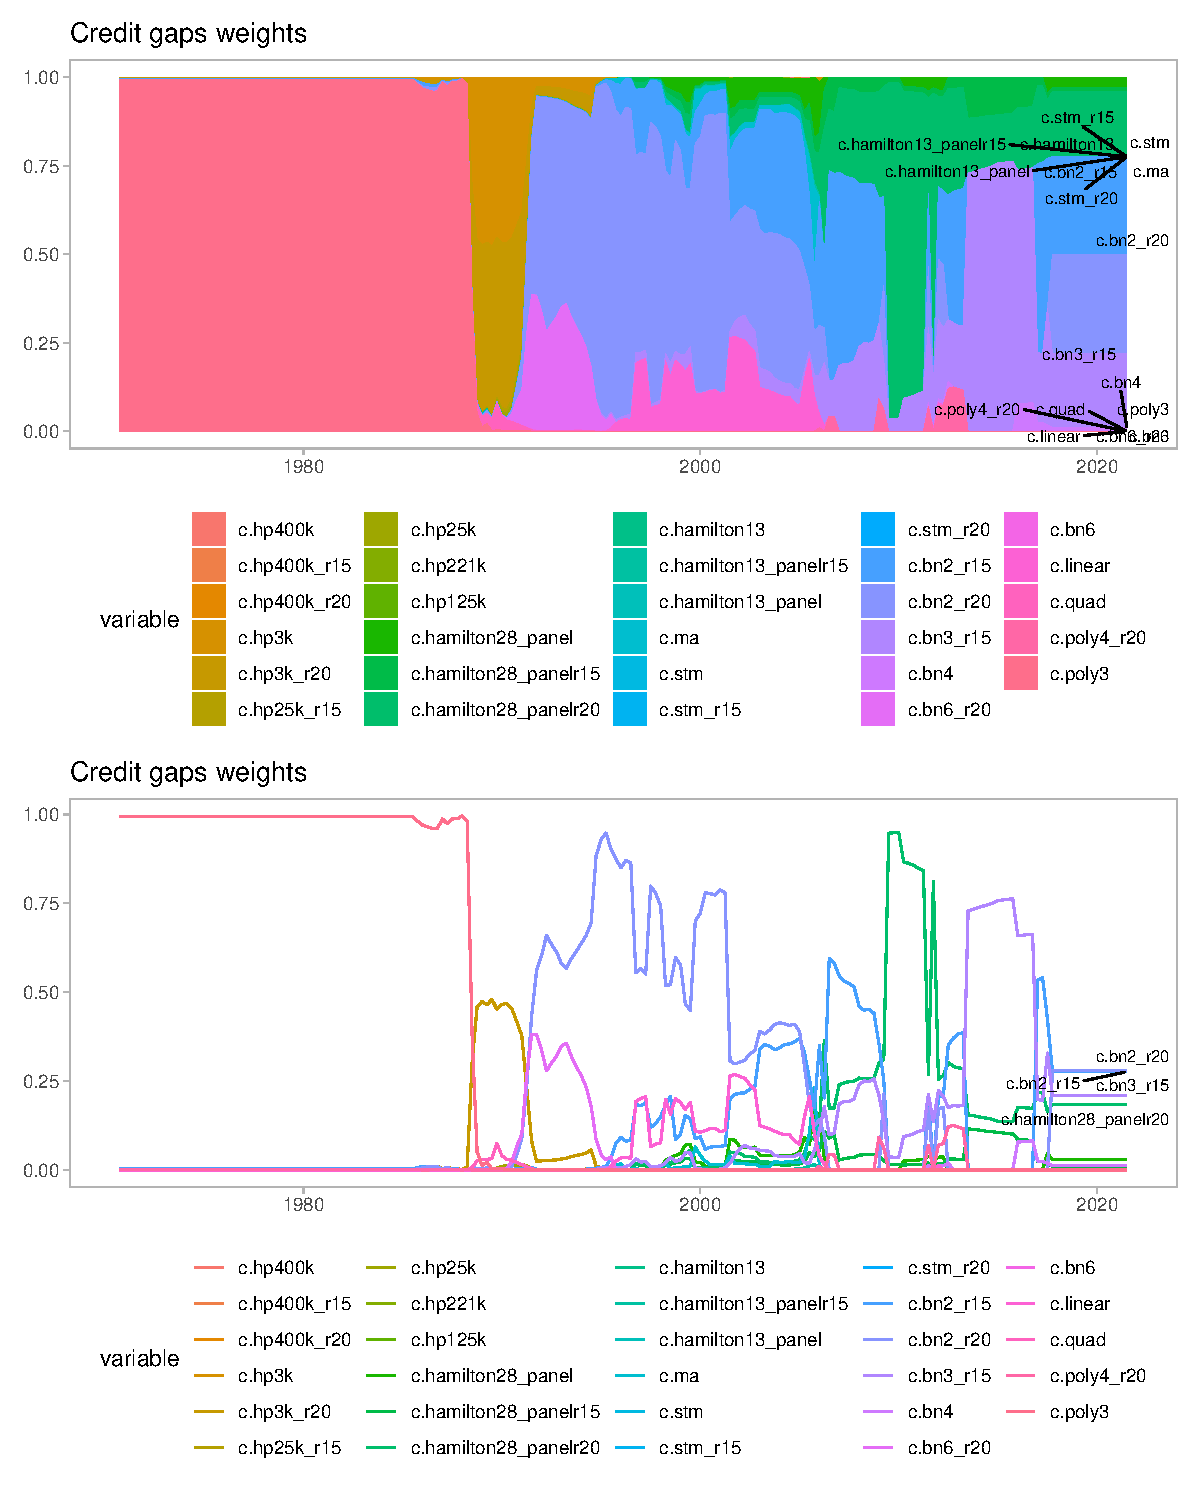
\includegraphics[width=1\linewidth]{../Data/Output/Graphs/Weights_combined} 

}

\caption{One sided weights graph}\label{fig:weightgraph}
\end{figure}

\hypertarget{empirical-results}{%
\section{Empirical Results}\label{empirical-results}}

\hypertarget{weight-graphs}{%
\subsection{One sided weights stacked time series graph}\label{weight-graphs}}

In Figure \ref{fig:weightgraph}, we see that for the first 15-18 years of the data sample, the parsimony (c.poly3) filter's weight dominated all the other filters. However, after about 20 years, the (c.poly3) filter lost all of its weight. This could be explained by the lack of initial data, leading to poorer performance of other credit gap measurements.

However, as more data were updated, the dynamics of the weights changed significantly. During the early 1990s, Hodrick-Prescott filters' weights overshadowed others, then Beveridge-Nelson, and the Structural Time-Series model did. As the Great Financial Crisis happened, the Hamilton filter in a panel setting gained weight. And lastly, at the end of the crisis data period 2017:Q4, we have 3 Beveridge-Nelson filters (c.bn2\_r20, c.bn2\_r15 and c.bn3\_r15) and 1 Hamilton filter (c.hamiolton28\_panelr20) sharing nearly equal weights. To apply our findings in our limited sample, we fixed the weights for 2017:Q4 at constant and extrapolated the weights to 2021:Q3, the end of this paper's credit data availability.

\hypertarget{model-fit}{%
\subsection{Model Fitness Results}\label{model-fit}}

The standard deviation for each estimate is deducted from a 95\% confidence interval of the bootstrapping results using 2000 stratified bootstrap replicates.\footnote{We estimate partial ROC and confidence interval using the R package ``pROC'' by Robin et al. (\protect\hyperlink{ref-robin_proc_2011}{2011}) whose methodology is based on Carpenter \& Bithell (\protect\hyperlink{ref-carpenter_bootstrap_2000}{2000})}

\begin{table}[H]

\caption{\label{tab:varcompAE}Credit gaps performance as EWIs - Advanced Economies}
\centering
\resizebox{\linewidth}{!}{
\begin{tabular}[t]{llll>{}lllll}
\toprule
Cycle & BIC & AIC & AUC & psAUC & c.Threshold & Type I & Type II & Policy Loss Function\\
\midrule
\cellcolor{gray!6}{null} & \cellcolor{gray!6}{0.0000} & \cellcolor{gray!6}{0.0000} & \cellcolor{gray!6}{0.5000} & \textbf{\cellcolor{gray!6}{0.5000}} & \cellcolor{gray!6}{NA} & \cellcolor{gray!6}{1.0000} & \cellcolor{gray!6}{0.0000} & \cellcolor{gray!6}{1.0000}\\
 &  &  &  & \textbf{} &  &  &  & \\
\addlinespace
\textbf{\cellcolor{gray!6}{1.sided weighted.cycle}} & \textbf{\cellcolor{gray!6}{-128.8749}} & \textbf{\cellcolor{gray!6}{-134.9430}} & \textbf{\cellcolor{gray!6}{0.7545}} & \textbf{\textbf{\cellcolor{gray!6}{0.6889}}} & \textbf{\cellcolor{gray!6}{3.5486}} & \textbf{\cellcolor{gray!6}{0.3177}} & \textbf{\cellcolor{gray!6}{0.2841}} & \textbf{\cellcolor{gray!6}{0.1817}}\\
\textbf{} & \textbf{} & \textbf{} & \textbf{(0.0177)} & \textbf{\textbf{(0.0195)}} & \textbf{} & \textbf{(0.0088)} & \textbf{(0.0348)} & \textbf{(0.0254)}\\
\addlinespace
\cellcolor{gray!6}{c.hamilton13.panelr15} & \cellcolor{gray!6}{-116.9260} & \cellcolor{gray!6}{-122.9941} & \cellcolor{gray!6}{0.7282} & \textbf{\cellcolor{gray!6}{0.6846}} & \cellcolor{gray!6}{8.8000} & \cellcolor{gray!6}{0.3469} & \cellcolor{gray!6}{0.3011} & \cellcolor{gray!6}{0.2110}\\
 &  &  & (0.0174) & \textbf{(0.0178)} &  & (0.0087) & (0.0348) & (0.0270)\\
\addlinespace
\cellcolor{gray!6}{c.hamilton28.panelr15} & \cellcolor{gray!6}{-141.5772} & \cellcolor{gray!6}{-147.6453} & \cellcolor{gray!6}{0.7491} & \textbf{\cellcolor{gray!6}{0.6825}} & \cellcolor{gray!6}{11.5510} & \cellcolor{gray!6}{0.3834} & \cellcolor{gray!6}{0.2216} & \cellcolor{gray!6}{0.1961}\\
 &  &  & (0.0184) & \textbf{(0.0198)} &  & (0.0088) & (0.0319) & (0.0212)\\
\addlinespace
\cellcolor{gray!6}{c.hamilton28.panelr20} & \cellcolor{gray!6}{-147.4322} & \cellcolor{gray!6}{-153.5003} & \cellcolor{gray!6}{0.7514} & \textbf{\cellcolor{gray!6}{0.6811}} & \cellcolor{gray!6}{13.1072} & \cellcolor{gray!6}{0.3489} & \cellcolor{gray!6}{0.2898} & \cellcolor{gray!6}{0.2057}\\
 &  &  & (0.0185) & \textbf{(0.0195)} &  & (0.0086) & (0.0348) & (0.0262)\\
\addlinespace
\cellcolor{gray!6}{c.bn6.r20} & \cellcolor{gray!6}{-90.1022} & \cellcolor{gray!6}{-96.1703} & \cellcolor{gray!6}{0.7338} & \textbf{\cellcolor{gray!6}{0.6751}} & \cellcolor{gray!6}{0.6581} & \cellcolor{gray!6}{0.4126} & \cellcolor{gray!6}{0.2273} & \cellcolor{gray!6}{0.2219}\\
 &  &  & (0.0183) & \textbf{(0.0171)} &  & (0.0094) & (0.0319) & (0.0222)\\
\addlinespace
\cellcolor{gray!6}{c.hamilton28.panel} & \cellcolor{gray!6}{-129.1730} & \cellcolor{gray!6}{-135.2411} & \cellcolor{gray!6}{0.7382} & \textbf{\cellcolor{gray!6}{0.6740}} & \cellcolor{gray!6}{9.7674} & \cellcolor{gray!6}{0.3977} & \cellcolor{gray!6}{0.2386} & \cellcolor{gray!6}{0.2151}\\
 &  &  & (0.0187) & \textbf{(0.0189)} &  & (0.0090) & (0.0319) & (0.0224)\\
\addlinespace
\cellcolor{gray!6}{c.hamilton13.panel} & \cellcolor{gray!6}{-122.0054} & \cellcolor{gray!6}{-128.0735} & \cellcolor{gray!6}{0.7208} & \textbf{\cellcolor{gray!6}{0.6684}} & \cellcolor{gray!6}{7.2247} & \cellcolor{gray!6}{0.3509} & \cellcolor{gray!6}{0.3239} & \cellcolor{gray!6}{0.2280}\\
 &  &  & (0.0182) & \textbf{(0.0174)} &  & (0.0090) & (0.0362) & (0.0296)\\
\addlinespace
\cellcolor{gray!6}{c.ma} & \cellcolor{gray!6}{-97.4868} & \cellcolor{gray!6}{-103.5549} & \cellcolor{gray!6}{0.7133} & \textbf{\cellcolor{gray!6}{0.6677}} & \cellcolor{gray!6}{6.0375} & \cellcolor{gray!6}{0.4073} & \cellcolor{gray!6}{0.2727} & \cellcolor{gray!6}{0.2403}\\
 &  &  & (0.0181) & \textbf{(0.0174)} &  & (0.0087) & (0.0333) & (0.0255)\\
\addlinespace
\cellcolor{gray!6}{c.bn6} & \cellcolor{gray!6}{-104.1404} & \cellcolor{gray!6}{-110.2085} & \cellcolor{gray!6}{0.7042} & \textbf{\cellcolor{gray!6}{0.6426}} & \cellcolor{gray!6}{0.8256} & \cellcolor{gray!6}{0.4040} & \cellcolor{gray!6}{0.2955} & \cellcolor{gray!6}{0.2505}\\
 &  &  & (0.0198) & \textbf{(0.0184)} &  & (0.0089) & (0.0348) & (0.0277)\\
\addlinespace
\cellcolor{gray!6}{c.hp125k} & \cellcolor{gray!6}{-92.8331} & \cellcolor{gray!6}{-98.9012} & \cellcolor{gray!6}{0.6977} & \textbf{\cellcolor{gray!6}{0.6397}} & \cellcolor{gray!6}{3.6972} & \cellcolor{gray!6}{0.3788} & \cellcolor{gray!6}{0.3239} & \cellcolor{gray!6}{0.2484}\\
 &  &  & (0.0195) & \textbf{(0.0185)} &  & (0.0089) & (0.0348) & (0.0293)\\
\addlinespace
\textbf{\cellcolor{gray!6}{BIS Basel gap}} & \textbf{\cellcolor{gray!6}{-113.9826}} & \textbf{\cellcolor{gray!6}{-120.0507}} & \textbf{\cellcolor{gray!6}{0.7124}} & \textbf{\textbf{\cellcolor{gray!6}{0.6390}}} & \textbf{\cellcolor{gray!6}{3.9706}} & \textbf{\cellcolor{gray!6}{0.3847}} & \textbf{\cellcolor{gray!6}{0.3011}} & \textbf{\cellcolor{gray!6}{0.2387}}\\
\textbf{} & \textbf{} & \textbf{} & \textbf{(0.0200)} & \textbf{\textbf{(0.0197)}} & \textbf{} & \textbf{(0.0085)} & \textbf{(0.0348)} & \textbf{(0.0275)}\\
\addlinespace
\cellcolor{gray!6}{c.hp221k} & \cellcolor{gray!6}{-104.1190} & \cellcolor{gray!6}{-110.1871} & \cellcolor{gray!6}{0.7070} & \textbf{\cellcolor{gray!6}{0.6388}} & \cellcolor{gray!6}{3.8869} & \cellcolor{gray!6}{0.3755} & \cellcolor{gray!6}{0.3011} & \cellcolor{gray!6}{0.2317}\\
 &  &  & (0.0198) & \textbf{(0.0197)} &  & (0.0086) & (0.0362) & (0.0285)\\
\addlinespace
\cellcolor{gray!6}{c.stm.r15} & \cellcolor{gray!6}{-86.6063} & \cellcolor{gray!6}{-92.6744} & \cellcolor{gray!6}{0.6989} & \textbf{\cellcolor{gray!6}{0.6382}} & \cellcolor{gray!6}{4.0784} & \cellcolor{gray!6}{0.3486} & \cellcolor{gray!6}{0.3295} & \cellcolor{gray!6}{0.2301}\\
 &  &  & (0.0195) & \textbf{(0.0204)} &  & (0.0090) & (0.0348) & (0.0292)\\
\addlinespace
\cellcolor{gray!6}{c.stm} & \cellcolor{gray!6}{-89.9073} & \cellcolor{gray!6}{-95.9754} & \cellcolor{gray!6}{0.6929} & \textbf{\cellcolor{gray!6}{0.6357}} & \cellcolor{gray!6}{3.3071} & \cellcolor{gray!6}{0.3924} & \cellcolor{gray!6}{0.3295} & \cellcolor{gray!6}{0.2626}\\
 &  &  & (0.0197) & \textbf{(0.0193)} &  & (0.0091) & (0.0348) & (0.0300)\\
\addlinespace
\cellcolor{gray!6}{c.hp400k.r15} & \cellcolor{gray!6}{-73.5902} & \cellcolor{gray!6}{-79.6582} & \cellcolor{gray!6}{0.6869} & \textbf{\cellcolor{gray!6}{0.6357}} & \cellcolor{gray!6}{4.2355} & \cellcolor{gray!6}{0.3496} & \cellcolor{gray!6}{0.3125} & \cellcolor{gray!6}{0.2199}\\
 &  &  & (0.0194) & \textbf{(0.0201)} &  & (0.0085) & (0.0348) & (0.0277)\\
\addlinespace
\cellcolor{gray!6}{c.linear} & \cellcolor{gray!6}{-111.9570} & \cellcolor{gray!6}{-118.0251} & \cellcolor{gray!6}{0.7069} & \textbf{\cellcolor{gray!6}{0.6356}} & \cellcolor{gray!6}{3.9964} & \cellcolor{gray!6}{0.4620} & \cellcolor{gray!6}{0.2443} & \cellcolor{gray!6}{0.2732}\\
 &  &  & (0.0206) & \textbf{(0.0177)} &  & (0.0092) & (0.0319) & (0.0241)\\
\addlinespace
\cellcolor{gray!6}{c.hp400k.r20} & \cellcolor{gray!6}{-93.8576} & \cellcolor{gray!6}{-99.9257} & \cellcolor{gray!6}{0.6991} & \textbf{\cellcolor{gray!6}{0.6340}} & \cellcolor{gray!6}{4.3393} & \cellcolor{gray!6}{0.3622} & \cellcolor{gray!6}{0.3295} & \cellcolor{gray!6}{0.2398}\\
 &  &  & (0.0197) & \textbf{(0.0197)} &  & (0.0090) & (0.0362) & (0.0306)\\
\addlinespace
\cellcolor{gray!6}{c.bn2.r20} & \cellcolor{gray!6}{-84.0800} & \cellcolor{gray!6}{-90.1481} & \cellcolor{gray!6}{0.6955} & \textbf{\cellcolor{gray!6}{0.6297}} & \cellcolor{gray!6}{0.2773} & \cellcolor{gray!6}{0.4216} & \cellcolor{gray!6}{0.3182} & \cellcolor{gray!6}{0.2790}\\
 &  &  & (0.0201) & \textbf{(0.0168)} &  & (0.0090) & (0.0348) & (0.0301)\\
\addlinespace
\cellcolor{gray!6}{c.stm.r20} & \cellcolor{gray!6}{-87.6992} & \cellcolor{gray!6}{-93.7673} & \cellcolor{gray!6}{0.6879} & \textbf{\cellcolor{gray!6}{0.6282}} & \cellcolor{gray!6}{3.1055} & \cellcolor{gray!6}{0.4073} & \cellcolor{gray!6}{0.3239} & \cellcolor{gray!6}{0.2708}\\
 &  &  & (0.0200) & \textbf{(0.0178)} &  & (0.0089) & (0.0348) & (0.0298)\\
\bottomrule
\multicolumn{9}{l}{\textsuperscript{} The standard deviation for each estimates are deducted from 95\% confidence interval of the bootstrapping results}\\
\multicolumn{9}{l}{using 2000 stratified bootstrap replicates.}\\
\end{tabular}}
\end{table}

\begin{table}[H]

\caption{\label{tab:varcompEME}Credit gaps performance as EWIs - Emerging Market Economies}
\centering
\resizebox{\linewidth}{!}{
\begin{tabular}[t]{llll>{}lllll}
\toprule
Cycle & BIC & AIC & AUC & psAUC & c.Threshold & Type I & Type II & Policy Loss Function\\
\midrule
\cellcolor{gray!6}{null} & \cellcolor{gray!6}{0.0000} & \cellcolor{gray!6}{0.0000} & \cellcolor{gray!6}{0.5000} & \textbf{\cellcolor{gray!6}{0.5000}} & \cellcolor{gray!6}{NA} & \cellcolor{gray!6}{1.0000} & \cellcolor{gray!6}{0.0000} & \cellcolor{gray!6}{1.0000}\\
 &  &  &  & \textbf{} &  &  &  & \\
\addlinespace
\cellcolor{gray!6}{c.bn3.r15} & \cellcolor{gray!6}{-46.2774} & \cellcolor{gray!6}{-51.3507} & \cellcolor{gray!6}{0.7365} & \textbf{\cellcolor{gray!6}{0.6308}} & \cellcolor{gray!6}{0.6244} & \cellcolor{gray!6}{0.3059} & \cellcolor{gray!6}{0.3333} & \cellcolor{gray!6}{0.2047}\\
 &  &  & (0.0471) & \textbf{(0.0451)} &  & (0.0134) & (0.0779) & (0.0623)\\
\addlinespace
\cellcolor{gray!6}{c.poly3} & \cellcolor{gray!6}{5.3862} & \cellcolor{gray!6}{0.3129} & \cellcolor{gray!6}{0.5737} & \textbf{\cellcolor{gray!6}{0.6046}} & \cellcolor{gray!6}{1.8089} & \cellcolor{gray!6}{0.5280} & \cellcolor{gray!6}{0.3056} & \cellcolor{gray!6}{0.3721}\\
 &  &  & (0.0358) & \textbf{(0.0264)} &  & (0.0152) & (0.0709) & (0.0593)\\
\addlinespace
\cellcolor{gray!6}{c.bn2.r15} & \cellcolor{gray!6}{-13.2062} & \cellcolor{gray!6}{-18.2795} & \cellcolor{gray!6}{0.6879} & \textbf{\cellcolor{gray!6}{0.5879}} & \cellcolor{gray!6}{0.2952} & \cellcolor{gray!6}{0.3566} & \cellcolor{gray!6}{0.3333} & \cellcolor{gray!6}{0.2383}\\
 &  &  & (0.0505) & \textbf{(0.0508)} &  & (0.0140) & (0.0779) & (0.0642)\\
\addlinespace
\cellcolor{gray!6}{c.poly4.r20} & \cellcolor{gray!6}{7.0732} & \cellcolor{gray!6}{1.9999} & \cellcolor{gray!6}{0.5040} & \textbf{\cellcolor{gray!6}{0.5816}} & \cellcolor{gray!6}{-0.9609} & \cellcolor{gray!6}{0.5962} & \cellcolor{gray!6}{0.3333} & \cellcolor{gray!6}{0.4665}\\
 &  &  & (0.0339) & \textbf{(0.0160)} &  & (0.0147) & (0.0779) & (0.0717)\\
\addlinespace
\textbf{\cellcolor{gray!6}{1.sided weighted.cycle}} & \textbf{\cellcolor{gray!6}{6.2094}} & \textbf{\cellcolor{gray!6}{1.1361}} & \textbf{\cellcolor{gray!6}{0.5325}} & \textbf{\textbf{\cellcolor{gray!6}{0.5811}}} & \textbf{\cellcolor{gray!6}{-1.0639}} & \textbf{\cellcolor{gray!6}{0.6827}} & \textbf{\cellcolor{gray!6}{0.1111}} & \textbf{\cellcolor{gray!6}{0.4784}}\\
\textbf{} & \textbf{} & \textbf{} & \textbf{(0.0402)} & \textbf{\textbf{(0.0183)}} & \textbf{} & \textbf{(0.0136)} & \textbf{(0.0496)} & \textbf{(0.0310)}\\
\addlinespace
\cellcolor{gray!6}{c.linear} & \cellcolor{gray!6}{-9.3676} & \cellcolor{gray!6}{-14.4409} & \cellcolor{gray!6}{0.5787} & \textbf{\cellcolor{gray!6}{0.5774}} & \cellcolor{gray!6}{-0.9783} & \cellcolor{gray!6}{0.6294} & \cellcolor{gray!6}{0.2222} & \cellcolor{gray!6}{0.4455}\\
 &  &  & (0.0471) & \textbf{(0.0208)} &  & (0.0143) & (0.0709) & (0.0495)\\
\addlinespace
\cellcolor{gray!6}{c.bn2.r20} & \cellcolor{gray!6}{-16.6411} & \cellcolor{gray!6}{-21.7144} & \cellcolor{gray!6}{0.6760} & \textbf{\cellcolor{gray!6}{0.5751}} & \cellcolor{gray!6}{0.1470} & \cellcolor{gray!6}{0.4510} & \cellcolor{gray!6}{0.3056} & \cellcolor{gray!6}{0.2968}\\
 &  &  & (0.0519) & \textbf{(0.0462)} &  & (0.0154) & (0.0709) & (0.0572)\\
\addlinespace
\cellcolor{gray!6}{c.hamilton13} & \cellcolor{gray!6}{6.5749} & \cellcolor{gray!6}{1.5016} & \cellcolor{gray!6}{0.5468} & \textbf{\cellcolor{gray!6}{0.5710}} & \cellcolor{gray!6}{3.6354} & \cellcolor{gray!6}{0.6206} & \cellcolor{gray!6}{0.3056} & \cellcolor{gray!6}{0.4785}\\
 &  &  & (0.0386) & \textbf{(0.0229)} &  & (0.0143) & (0.0709) & (0.0610)\\
\addlinespace
\cellcolor{gray!6}{c.ma} & \cellcolor{gray!6}{-11.6401} & \cellcolor{gray!6}{-16.7133} & \cellcolor{gray!6}{0.5572} & \textbf{\cellcolor{gray!6}{0.5457}} & \cellcolor{gray!6}{-0.2250} & \cellcolor{gray!6}{0.7220} & \cellcolor{gray!6}{0.1667} & \cellcolor{gray!6}{0.5491}\\
 &  &  & (0.0546) & \textbf{(0.0164)} &  & (0.0134) & (0.0567) & (0.0382)\\
\addlinespace
\cellcolor{gray!6}{c.hamilton28.panel} & \cellcolor{gray!6}{-7.8687} & \cellcolor{gray!6}{-12.9420} & \cellcolor{gray!6}{0.5392} & \textbf{\cellcolor{gray!6}{0.5384}} & \cellcolor{gray!6}{-1.7750} & \cellcolor{gray!6}{0.6958} & \cellcolor{gray!6}{0.2778} & \cellcolor{gray!6}{0.5613}\\
 &  &  & (0.0522) & \textbf{(0.0170)} &  & (0.0132) & (0.0709) & (0.0577)\\
\addlinespace
\cellcolor{gray!6}{c.quad} & \cellcolor{gray!6}{6.1997} & \cellcolor{gray!6}{1.1264} & \cellcolor{gray!6}{0.4654} & \textbf{\cellcolor{gray!6}{0.5334}} & \cellcolor{gray!6}{-6.4882} & \cellcolor{gray!6}{0.7456} & \cellcolor{gray!6}{0.1944} & \cellcolor{gray!6}{0.5938}\\
 &  &  & (0.0474) & \textbf{(0.0140)} &  & (0.0127) & (0.0638) & (0.0455)\\
\addlinespace
\cellcolor{gray!6}{c.hamilton13.panelr15} & \cellcolor{gray!6}{-1.6660} & \cellcolor{gray!6}{-6.7393} & \cellcolor{gray!6}{0.5087} & \textbf{\cellcolor{gray!6}{0.5274}} & \cellcolor{gray!6}{-1.1064} & \cellcolor{gray!6}{0.7002} & \cellcolor{gray!6}{0.3333} & \cellcolor{gray!6}{0.6014}\\
 &  &  & (0.0550) & \textbf{(0.0130)} &  & (0.0136) & (0.0779) & (0.0732)\\
\addlinespace
\cellcolor{gray!6}{c.hp25k.r15} & \cellcolor{gray!6}{3.6420} & \cellcolor{gray!6}{-1.4313} & \cellcolor{gray!6}{0.5018} & \textbf{\cellcolor{gray!6}{0.5265}} & \cellcolor{gray!6}{-3.5672} & \cellcolor{gray!6}{0.7850} & \cellcolor{gray!6}{0.1111} & \cellcolor{gray!6}{0.6285}\\
 &  &  & (0.0558) & \textbf{(0.0101)} &  & (0.0125) & (0.0496) & (0.0320)\\
\addlinespace
\cellcolor{gray!6}{c.hp25k} & \cellcolor{gray!6}{3.9466} & \cellcolor{gray!6}{-1.1267} & \cellcolor{gray!6}{0.4975} & \textbf{\cellcolor{gray!6}{0.5247}} & \cellcolor{gray!6}{-3.7339} & \cellcolor{gray!6}{0.7893} & \cellcolor{gray!6}{0.1111} & \cellcolor{gray!6}{0.6354}\\
 &  &  & (0.0560) & \textbf{(0.0099)} &  & (0.0118) & (0.0496) & (0.0310)\\
\addlinespace
\cellcolor{gray!6}{c.hp3k} & \cellcolor{gray!6}{3.3678} & \cellcolor{gray!6}{-1.7054} & \cellcolor{gray!6}{0.5276} & \textbf{\cellcolor{gray!6}{0.5235}} & \cellcolor{gray!6}{-1.1119} & \cellcolor{gray!6}{0.7019} & \cellcolor{gray!6}{0.3333} & \cellcolor{gray!6}{0.6038}\\
 &  &  & (0.0556) & \textbf{(0.0146)} &  & (0.0136) & (0.0850) & (0.0758)\\
\addlinespace
\cellcolor{gray!6}{c.hp3k.r20} & \cellcolor{gray!6}{3.3703} & \cellcolor{gray!6}{-1.7030} & \cellcolor{gray!6}{0.5276} & \textbf{\cellcolor{gray!6}{0.5235}} & \cellcolor{gray!6}{-1.1125} & \cellcolor{gray!6}{0.7028} & \cellcolor{gray!6}{0.3333} & \cellcolor{gray!6}{0.6050}\\
 &  &  & (0.0556) & \textbf{(0.0149)} &  & (0.0132) & (0.0779) & (0.0726)\\
\addlinespace
\cellcolor{gray!6}{c.hamilton13.panel} & \cellcolor{gray!6}{-1.6294} & \cellcolor{gray!6}{-6.7027} & \cellcolor{gray!6}{0.5166} & \textbf{\cellcolor{gray!6}{0.5222}} & \cellcolor{gray!6}{-2.9398} & \cellcolor{gray!6}{0.7500} & \cellcolor{gray!6}{0.2778} & \cellcolor{gray!6}{0.6397}\\
 &  &  & (0.0554) & \textbf{(0.0134)} &  & (0.0132) & (0.0709) & (0.0591)\\
\addlinespace
\textbf{\cellcolor{gray!6}{BIS Basel gap}} & \textbf{\cellcolor{gray!6}{-0.7015}} & \textbf{\cellcolor{gray!6}{-5.7748}} & \textbf{\cellcolor{gray!6}{0.4928}} & \textbf{\textbf{\cellcolor{gray!6}{0.5217}}} & \textbf{\cellcolor{gray!6}{-5.3969}} & \textbf{\cellcolor{gray!6}{0.7920}} & \textbf{\cellcolor{gray!6}{0.1389}} & \textbf{\cellcolor{gray!6}{0.6465}}\\
\textbf{} & \textbf{} & \textbf{} & \textbf{(0.0544)} & \textbf{\textbf{(0.0100)}} & \textbf{} & \textbf{(0.0118)} & \textbf{(0.0638)} & \textbf{(0.0382)}\\
\addlinespace
\cellcolor{gray!6}{c.hamilton28.panelr20} & \cellcolor{gray!6}{-4.9986} & \cellcolor{gray!6}{-10.0719} & \cellcolor{gray!6}{0.5123} & \textbf{\cellcolor{gray!6}{0.5213}} & \cellcolor{gray!6}{-1.5578} & \cellcolor{gray!6}{0.6932} & \cellcolor{gray!6}{0.3333} & \cellcolor{gray!6}{0.5916}\\
 &  &  & (0.0544) & \textbf{(0.0147)} &  & (0.0136) & (0.0710) & (0.0663)\\
\bottomrule
\multicolumn{9}{l}{\textsuperscript{} The standard deviation for each estimates are deducted from 95\% confidence interval of the bootstrapping}\\
\multicolumn{9}{l}{results using 2000 stratified bootstrap replicates.}\\
\end{tabular}}
\end{table}

\begin{table}[H]

\caption{\label{tab:varcompfull}Credit gaps performance as EWIs comparison - Full sample}
\centering
\resizebox{\linewidth}{!}{
\begin{tabular}[t]{llll>{}lllll}
\toprule
Cycle & BIC & AIC & AUC & psAUC & c.Threshold & Type I & Type II & Policy Loss Function\\
\midrule
\cellcolor{gray!6}{null} & \cellcolor{gray!6}{0.0000} & \cellcolor{gray!6}{0.0000} & \cellcolor{gray!6}{0.5000} & \textbf{\cellcolor{gray!6}{0.5000}} & \cellcolor{gray!6}{NA} & \cellcolor{gray!6}{1.0000} & \cellcolor{gray!6}{0.0000} & \cellcolor{gray!6}{1.0000}\\
 &  &  &  & \textbf{} &  &  &  & \\
\addlinespace
\textbf{\cellcolor{gray!6}{1.sided weighted.cycle}} & \textbf{\cellcolor{gray!6}{-127.5308}} & \textbf{\cellcolor{gray!6}{-133.9135}} & \textbf{\cellcolor{gray!6}{0.7182}} & \textbf{\textbf{\cellcolor{gray!6}{0.6454}}} & \textbf{\cellcolor{gray!6}{2.8892}} & \textbf{\cellcolor{gray!6}{0.3532}} & \textbf{\cellcolor{gray!6}{0.3255}} & \textbf{\cellcolor{gray!6}{0.2307}}\\
\textbf{} & \textbf{} & \textbf{} & \textbf{(0.0174)} & \textbf{\textbf{(0.0165)}} & \textbf{} & \textbf{(0.0076)} & \textbf{(0.0313)} & \textbf{(0.0257)}\\
\addlinespace
\cellcolor{gray!6}{c.bn6.r20} & \cellcolor{gray!6}{-108.0679} & \cellcolor{gray!6}{-114.4506} & \cellcolor{gray!6}{0.7048} & \textbf{\cellcolor{gray!6}{0.6379}} & \cellcolor{gray!6}{0.6581} & \cellcolor{gray!6}{0.3962} & \cellcolor{gray!6}{0.3019} & \cellcolor{gray!6}{0.2481}\\
 &  &  & (0.0184) & \textbf{(0.0176)} &  & (0.0077) & (0.0313) & (0.0250)\\
\addlinespace
\cellcolor{gray!6}{c.hamilton28.panel} & \cellcolor{gray!6}{-149.8518} & \cellcolor{gray!6}{-156.2346} & \cellcolor{gray!6}{0.7107} & \textbf{\cellcolor{gray!6}{0.6359}} & \cellcolor{gray!6}{9.7674} & \cellcolor{gray!6}{0.3912} & \cellcolor{gray!6}{0.3066} & \cellcolor{gray!6}{0.2470}\\
 &  &  & (0.0185) & \textbf{(0.0169)} &  & (0.0075) & (0.0313) & (0.0251)\\
\addlinespace
\cellcolor{gray!6}{c.ma} & \cellcolor{gray!6}{-120.8108} & \cellcolor{gray!6}{-127.1936} & \cellcolor{gray!6}{0.6922} & \textbf{\cellcolor{gray!6}{0.6313}} & \cellcolor{gray!6}{5.7813} & \cellcolor{gray!6}{0.3989} & \cellcolor{gray!6}{0.3160} & \cellcolor{gray!6}{0.2590}\\
 &  &  & (0.0181) & \textbf{(0.0170)} &  & (0.0077) & (0.0313) & (0.0259)\\
\addlinespace
\cellcolor{gray!6}{c.hamilton13.panelr15} & \cellcolor{gray!6}{-126.2968} & \cellcolor{gray!6}{-132.6796} & \cellcolor{gray!6}{0.6924} & \textbf{\cellcolor{gray!6}{0.6311}} & \cellcolor{gray!6}{6.5289} & \cellcolor{gray!6}{0.4297} & \cellcolor{gray!6}{0.2830} & \cellcolor{gray!6}{0.2647}\\
 &  &  & (0.0180) & \textbf{(0.0175)} &  & (0.0079) & (0.0313) & (0.0245)\\
\addlinespace
\cellcolor{gray!6}{c.hamilton28.panelr20} & \cellcolor{gray!6}{-164.6015} & \cellcolor{gray!6}{-170.9842} & \cellcolor{gray!6}{0.7158} & \textbf{\cellcolor{gray!6}{0.6302}} & \cellcolor{gray!6}{10.8558} & \cellcolor{gray!6}{0.3948} & \cellcolor{gray!6}{0.2925} & \cellcolor{gray!6}{0.2414}\\
 &  &  & (0.0189) & \textbf{(0.0181)} &  & (0.0074) & (0.0313) & (0.0241)\\
\addlinespace
\cellcolor{gray!6}{c.hamilton28.panelr15} & \cellcolor{gray!6}{-154.4533} & \cellcolor{gray!6}{-160.8361} & \cellcolor{gray!6}{0.7091} & \textbf{\cellcolor{gray!6}{0.6270}} & \cellcolor{gray!6}{11.5510} & \cellcolor{gray!6}{0.3854} & \cellcolor{gray!6}{0.2972} & \cellcolor{gray!6}{0.2369}\\
 &  &  & (0.0190) & \textbf{(0.0184)} &  & (0.0077) & (0.0325) & (0.0254)\\
\addlinespace
\cellcolor{gray!6}{c.hamilton13.panel} & \cellcolor{gray!6}{-133.9347} & \cellcolor{gray!6}{-140.3175} & \cellcolor{gray!6}{0.6922} & \textbf{\cellcolor{gray!6}{0.6250}} & \cellcolor{gray!6}{4.9769} & \cellcolor{gray!6}{0.4285} & \cellcolor{gray!6}{0.2877} & \cellcolor{gray!6}{0.2664}\\
 &  &  & (0.0184) & \textbf{(0.0169)} &  & (0.0075) & (0.0301) & (0.0239)\\
\addlinespace
\cellcolor{gray!6}{c.bn2.r20} & \cellcolor{gray!6}{-109.3128} & \cellcolor{gray!6}{-115.6955} & \cellcolor{gray!6}{0.6963} & \textbf{\cellcolor{gray!6}{0.6218}} & \cellcolor{gray!6}{0.2776} & \cellcolor{gray!6}{0.4080} & \cellcolor{gray!6}{0.3255} & \cellcolor{gray!6}{0.2724}\\
 &  &  & (0.0188) & \textbf{(0.0170)} &  & (0.0079) & (0.0313) & (0.0268)\\
\addlinespace
\cellcolor{gray!6}{c.linear} & \cellcolor{gray!6}{-135.4069} & \cellcolor{gray!6}{-141.7896} & \cellcolor{gray!6}{0.6879} & \textbf{\cellcolor{gray!6}{0.6204}} & \cellcolor{gray!6}{3.9989} & \cellcolor{gray!6}{0.4616} & \cellcolor{gray!6}{0.2925} & \cellcolor{gray!6}{0.2986}\\
 &  &  & (0.0191) & \textbf{(0.0145)} &  & (0.0079) & (0.0325) & (0.0264)\\
\addlinespace
\cellcolor{gray!6}{c.bn6} & \cellcolor{gray!6}{-132.7915} & \cellcolor{gray!6}{-139.1742} & \cellcolor{gray!6}{0.6835} & \textbf{\cellcolor{gray!6}{0.6113}} & \cellcolor{gray!6}{0.4710} & \cellcolor{gray!6}{0.4371} & \cellcolor{gray!6}{0.2830} & \cellcolor{gray!6}{0.2712}\\
 &  &  & (0.0194) & \textbf{(0.0188)} &  & (0.0075) & (0.0313) & (0.0242)\\
\addlinespace
\cellcolor{gray!6}{c.bn2.r15} & \cellcolor{gray!6}{-83.9469} & \cellcolor{gray!6}{-90.3297} & \cellcolor{gray!6}{0.6749} & \textbf{\cellcolor{gray!6}{0.6047}} & \cellcolor{gray!6}{0.1349} & \cellcolor{gray!6}{0.4761} & \cellcolor{gray!6}{0.3302} & \cellcolor{gray!6}{0.3357}\\
 &  &  & (0.0192) & \textbf{(0.0149)} &  & (0.0074) & (0.0313) & (0.0277)\\
\addlinespace
\cellcolor{gray!6}{c.poly4.r20} & \cellcolor{gray!6}{3.5738} & \cellcolor{gray!6}{-2.8090} & \cellcolor{gray!6}{0.5772} & \textbf{\cellcolor{gray!6}{0.6011}} & \cellcolor{gray!6}{0.1651} & \cellcolor{gray!6}{0.4980} & \cellcolor{gray!6}{0.3302} & \cellcolor{gray!6}{0.3570}\\
 &  &  & (0.0154) & \textbf{(0.0144)} &  & (0.0077) & (0.0313) & (0.0284)\\
\addlinespace
\textbf{\cellcolor{gray!6}{BIS Basel gap}} & \textbf{\cellcolor{gray!6}{-121.5910}} & \textbf{\cellcolor{gray!6}{-127.9738}} & \textbf{\cellcolor{gray!6}{0.6733}} & \textbf{\textbf{\cellcolor{gray!6}{0.5960}}} & \textbf{\cellcolor{gray!6}{3.0578}} & \textbf{\cellcolor{gray!6}{0.4441}} & \textbf{\cellcolor{gray!6}{0.3255}} & \textbf{\cellcolor{gray!6}{0.3032}}\\
\textbf{} & \textbf{} & \textbf{} & \textbf{(0.0197)} & \textbf{\textbf{(0.0164)}} & \textbf{} & \textbf{(0.0077)} & \textbf{(0.0325)} & \textbf{(0.0281)}\\
\addlinespace
\cellcolor{gray!6}{c.bn4} & \cellcolor{gray!6}{-169.1186} & \cellcolor{gray!6}{-175.5014} & \cellcolor{gray!6}{0.6892} & \textbf{\cellcolor{gray!6}{0.5943}} & \cellcolor{gray!6}{1.2840} & \cellcolor{gray!6}{0.3837} & \cellcolor{gray!6}{0.3255} & \cellcolor{gray!6}{0.2532}\\
 &  &  & (0.0204) & \textbf{(0.0206)} &  & (0.0075) & (0.0325) & (0.0268)\\
\addlinespace
\cellcolor{gray!6}{c.stm.r15} & \cellcolor{gray!6}{-79.5531} & \cellcolor{gray!6}{-85.9358} & \cellcolor{gray!6}{0.6575} & \textbf{\cellcolor{gray!6}{0.5924}} & \cellcolor{gray!6}{2.0027} & \cellcolor{gray!6}{0.4778} & \cellcolor{gray!6}{0.3160} & \cellcolor{gray!6}{0.3281}\\
 &  &  & (0.0193) & \textbf{(0.0167)} &  & (0.0075) & (0.0325) & (0.0279)\\
\addlinespace
\cellcolor{gray!6}{c.hp125k} & \cellcolor{gray!6}{-92.2897} & \cellcolor{gray!6}{-98.6725} & \cellcolor{gray!6}{0.6562} & \textbf{\cellcolor{gray!6}{0.5924}} & \cellcolor{gray!6}{2.5216} & \cellcolor{gray!6}{0.4547} & \cellcolor{gray!6}{0.3302} & \cellcolor{gray!6}{0.3158}\\
 &  &  & (0.0194) & \textbf{(0.0164)} &  & (0.0077) & (0.0337) & (0.0293)\\
\addlinespace
\cellcolor{gray!6}{c.hp221k} & \cellcolor{gray!6}{-106.8842} & \cellcolor{gray!6}{-113.2670} & \cellcolor{gray!6}{0.6656} & \textbf{\cellcolor{gray!6}{0.5921}} & \cellcolor{gray!6}{2.6641} & \cellcolor{gray!6}{0.4561} & \cellcolor{gray!6}{0.3160} & \cellcolor{gray!6}{0.3079}\\
 &  &  & (0.0196) & \textbf{(0.0163)} &  & (0.0077) & (0.0325) & (0.0274)\\
\addlinespace
\cellcolor{gray!6}{c.hp400k.r15} & \cellcolor{gray!6}{-67.1228} & \cellcolor{gray!6}{-73.5055} & \cellcolor{gray!6}{0.6472} & \textbf{\cellcolor{gray!6}{0.5912}} & \cellcolor{gray!6}{2.6223} & \cellcolor{gray!6}{0.4592} & \cellcolor{gray!6}{0.3255} & \cellcolor{gray!6}{0.3168}\\
 &  &  & (0.0190) & \textbf{(0.0164)} &  & (0.0075) & (0.0313) & (0.0272)\\
\bottomrule
\multicolumn{9}{l}{\textsuperscript{} The standard deviation for each estimates are deducted from 95\% confidence interval of the bootstrapping results}\\
\multicolumn{9}{l}{using 2000 stratified bootstrap replicates.}\\
\end{tabular}}
\end{table}

\hypertarget{performance-metrics}{%
\subsubsection{Performance Metrics}\label{performance-metrics}}

Along with the results from Table \ref{tab:varcompAE} - \ref{tab:varcompfull}, we will discuss psAUC as a performance measurement criteria of a credit gap series as an EWI.

Firstly, the psAUC metric overall gives a consistent signal about the quality of the credit gap decomposition filters. A filter with a higher psAUC value, in general, will have a higher quality set of possible policy loss function values to optimize. The standard deviation values of the weighted cycle metrics are also comparable to the other gap measurements.

In some scenarios, psAUC can be a deciding factor if policymakers are indifferent about the AUC value of a filter. In Table \ref{tab:varcompfull}, the Moving Average (c.ma) and Hamilton 13th lag using panel setting (c.hamilton13.panel) filters have the same AUC values. While the BIC and AIC values, the overall linearized binary logistic regression fitness criteria, would favor (c.hamilton13.panel) filter. The psAUC indicates otherwise. If we only focus on the region where FPR or the optimized threshold's predictive power is at least 2/3, the minimized policy loss function would favor c.ma.

However, there are also instances where psAUC failed to be a single criterion for determining the performance of a filter. In Table \ref{tab:varcompfull}, the 4th-degree polynomial filter with a rolling sample of 20 years (c.poly4.r20) have a higher psAUC value than the BIS Basel gap. However, all of (c.poly4.r20) filter's other metrics have less preferred values than the BIS Basel gap. As a result, we will deem (c.poly4.r20) less preferred than the BIS Basel gap.

In conclusion, even though psAUC is an overall good measurement for a specific case of binary regression model, where Type II errors are costlier than Type I errors, we focus our optimized threshold on the region where Type II errors are less than 1/3. We still have to use it in conjunction with other criteria such as BIC, AUC, and loss function to determine the performance of a filter. Using it alone will not give biased results of the model performance.

\hypertarget{weighted-gap-and-other-gaps-performance-comparison}{%
\subsubsection{Weighted gap and other gaps performance comparison}\label{weighted-gap-and-other-gaps-performance-comparison}}

In this part, we will discuss the performance of the weighted credit gap series as an EWI and compare it with other selected series.

From Table \ref{tab:varcompAE} and Table \ref{tab:varcompfull} regarding Advanced Economies and full sample results, the weighted credit cycle outperformed other cycles in AUC, psAUC, and Policy Loss function values. Specifically, while maintaining approximately the same optimized threshold as the BIS Basel gap, the weighted credit cycle can achieve lower Type I and II error rates than the BIS Basel gap in all samples.

The findings in Advanced Economies and full sample results also align with the literature findings. Hamilton, moving average filters with optimized parameters perform well, which agrees with the findings in Beltran et al. (\protect\hyperlink{ref-beltran_optimizing_2021}{2021}). Drehmann \& Yetman (\protect\hyperlink{ref-drehmann_which_2021}{2021}) proposed using Hamilton filter in a panel setting with fixed sloping coefficients across countries, and Galán (\protect\hyperlink{ref-galan_measuring_2019}{2019}) found rolling sample with 15 and 20 years window helps with improvement of the early indicator performance.

Across the three tables, optimizing and changing parameters on the one-sided HP filter does not improve its performance over the BIS Basel gap. Contrary to the finding in Beltran et al. (\protect\hyperlink{ref-beltran_optimizing_2021}{2021}) and Galán (\protect\hyperlink{ref-galan_measuring_2019}{2019}). The author did not use a full sample analysis but by individual countries. The structural time series filter proposed in Beltran et al. (\protect\hyperlink{ref-beltran_optimizing_2021}{2021}) also did not perform better than the BIS Basel gap.

Unsurprisingly, parsimony filters such as linear and polynomial does not perform well in AE and full sample. However, they can outperform other well-studied gaps in EMEs. This confirmed our finding in the previous section \ref{weight-graphs} that when data are limited, and the market economies are not well established, parsimony filters outperformed other complex filters.

We want to reiterate the importance of avoiding the pitfall of using a single criterion for selecting models, even for the psAUC metric. In Table \ref{tab:varcompEME}. The (c.poly3) filter has a higher psAUC value than its next filter on the table (c.bn2.r15). However, because (c.poly3)'s other metrics have lower quality than its counterpart, the policy loss function, Type I and II errors rates are higher for (c.poly3).

Last but not least, the emerging market economies (EMEs) have proven challenging to predict crises using the credit gap as EWI because of their more limited sample sizes and less established financial systems. Both Beltran et al. (\protect\hyperlink{ref-beltran_optimizing_2021}{2021}) and Drehmann \& Yetman (\protect\hyperlink{ref-drehmann_which_2021}{2021}) found that credit gap-based EWIs do not perform well in emerging market economies. In this paper, we found evidence that adding Beveridge-Nelson decomposition filters to the model selection process improved our model performance for the EMEs, specifically the (c.bn3.r15) Beveridge-Nelson with smoothing parameter 3 and 15 years rolling sample filter. Later graphical analysis in this paper on EMEs will include (c.bn3.r15) filter as another reference. Another Beveridge-Nelson filter with specific features such as (c.bn6.r20) also performs well in both AE and full samples.

\hypertarget{cross-validation}{%
\subsection{Out of sample forecast}\label{cross-validation}}

We followed Alessi \& Detken (\protect\hyperlink{ref-alessi_identifying_2018}{2018}) in implementing k-fold leave-one-out cross-validation to perform an out-of-sample forecast analysis. To assess the out-of-sample predictive power of the credit gaps, we perform a 3-fold cross-validation, in which the data is randomly split into three partitions. For each partition, the model is estimated using the other two groups. The resulting estimated parameter is then used to predict the dependent variable in the unused group. We then compute psAUCs and other metrics values and obtain the average metrics and their standard deviations from 10 repeats.

\begin{table}[H]

\caption{\label{tab:cvvarcompAE}Credit gaps performance as EWIs - Out of sample prediction - AE}
\centering
\resizebox{\linewidth}{!}{
\begin{tabular}[t]{lll>{}lllll}
\toprule
Cycle & BIC & AUC & psAUC & c.Threshold & Type I & Type II & Policy Loss Function\\
\midrule
\cellcolor{gray!6}{c.null} & \cellcolor{gray!6}{0.0000} & \cellcolor{gray!6}{0.4729} & \textbf{\cellcolor{gray!6}{0.4906}} & \cellcolor{gray!6}{0.0000} & \cellcolor{gray!6}{1.0000} & \cellcolor{gray!6}{0.0000} & \cellcolor{gray!6}{1.0000}\\
 & (1.4201) & (0.0099) & \textbf{(0.0032)} &  &  &  & \\
\addlinespace
\cellcolor{gray!6}{c.hamilton13.panelr15} & \cellcolor{gray!6}{-92.1757} & \cellcolor{gray!6}{0.7247} & \textbf{\cellcolor{gray!6}{0.6801}} & \cellcolor{gray!6}{8.0229} & \cellcolor{gray!6}{0.3694} & \cellcolor{gray!6}{0.2909} & \cellcolor{gray!6}{0.2220}\\
 & (3.1133) & (0.0050) & \textbf{(0.0053)} & (1.3409) & (0.0218) & (0.0245) & (0.0085)\\
\addlinespace
\textbf{\cellcolor{gray!6}{1.sided weighted.cycle}} & \textbf{\cellcolor{gray!6}{-83.3823}} & \textbf{\cellcolor{gray!6}{0.7469}} & \textbf{\textbf{\cellcolor{gray!6}{0.6776}}} & \textbf{\cellcolor{gray!6}{3.7972}} & \textbf{\cellcolor{gray!6}{0.3261}} & \textbf{\cellcolor{gray!6}{0.2915}} & \textbf{\cellcolor{gray!6}{0.1923}}\\
\textbf{} & \textbf{(5.0485)} & \textbf{(0.0084)} & \textbf{\textbf{(0.0127)}} & \textbf{(0.8036)} & \textbf{(0.0200)} & \textbf{(0.0253)} & \textbf{(0.0158)}\\
\addlinespace
\cellcolor{gray!6}{c.hamilton28.panelr15} & \cellcolor{gray!6}{-102.2043} & \cellcolor{gray!6}{0.7442} & \textbf{\cellcolor{gray!6}{0.6755}} & \cellcolor{gray!6}{12.1456} & \cellcolor{gray!6}{0.3595} & \cellcolor{gray!6}{0.2744} & \cellcolor{gray!6}{0.2058}\\
 & (3.1634) & (0.0036) & \textbf{(0.0059)} & (1.7511) & (0.0202) & (0.0300) & (0.0070)\\
\addlinespace
\cellcolor{gray!6}{c.hamilton28.panelr20} & \cellcolor{gray!6}{-106.5651} & \cellcolor{gray!6}{0.7469} & \textbf{\cellcolor{gray!6}{0.6748}} & \cellcolor{gray!6}{12.2954} & \cellcolor{gray!6}{0.3625} & \cellcolor{gray!6}{0.2722} & \cellcolor{gray!6}{0.2061}\\
 & (3.8537) & (0.0040) & \textbf{(0.0061)} & (1.8840) & (0.0151) & (0.0213) & (0.0037)\\
\addlinespace
\cellcolor{gray!6}{c.hamilton28.panel} & \cellcolor{gray!6}{-89.7510} & \cellcolor{gray!6}{0.7354} & \textbf{\cellcolor{gray!6}{0.6705}} & \cellcolor{gray!6}{10.0439} & \cellcolor{gray!6}{0.3930} & \cellcolor{gray!6}{0.2585} & \cellcolor{gray!6}{0.2220}\\
 & (2.9903) & (0.0024) & \textbf{(0.0036)} & (1.9885) & (0.0157) & (0.0226) & (0.0041)\\
\addlinespace
\cellcolor{gray!6}{c.hamilton13.panel} & \cellcolor{gray!6}{-101.4619} & \cellcolor{gray!6}{0.7184} & \textbf{\cellcolor{gray!6}{0.6665}} & \cellcolor{gray!6}{6.7644} & \cellcolor{gray!6}{0.3714} & \cellcolor{gray!6}{0.2983} & \cellcolor{gray!6}{0.2287}\\
 & (1.6108) & (0.0022) & \textbf{(0.0022)} & (1.0174) & (0.0260) & (0.0355) & (0.0039)\\
\addlinespace
\cellcolor{gray!6}{c.ma} & \cellcolor{gray!6}{-69.1570} & \cellcolor{gray!6}{0.7091} & \textbf{\cellcolor{gray!6}{0.6630}} & \cellcolor{gray!6}{6.0750} & \cellcolor{gray!6}{0.3994} & \cellcolor{gray!6}{0.2818} & \cellcolor{gray!6}{0.2410}\\
 & (3.2513) & (0.0036) & \textbf{(0.0051)} & (0.7204) & (0.0244) & (0.0405) & (0.0065)\\
\addlinespace
\cellcolor{gray!6}{c.bn6.r20} & \cellcolor{gray!6}{-72.3756} & \cellcolor{gray!6}{0.7062} & \textbf{\cellcolor{gray!6}{0.6353}} & \cellcolor{gray!6}{0.6105} & \cellcolor{gray!6}{0.4187} & \cellcolor{gray!6}{0.3028} & \cellcolor{gray!6}{0.2691}\\
 & (2.7401) & (0.0122) & \textbf{(0.0158)} & (1.4701) & (0.0333) & (0.0349) & (0.0324)\\
\addlinespace
\cellcolor{gray!6}{c.hp125k} & \cellcolor{gray!6}{-71.8112} & \cellcolor{gray!6}{0.6930} & \textbf{\cellcolor{gray!6}{0.6351}} & \cellcolor{gray!6}{3.5090} & \cellcolor{gray!6}{0.4030} & \cellcolor{gray!6}{0.3057} & \cellcolor{gray!6}{0.2568}\\
 & (5.1241) & (0.0039) & \textbf{(0.0030)} & (1.0440) & (0.0250) & (0.0217) & (0.0098)\\
\addlinespace
\textbf{\cellcolor{gray!6}{BIS Basel gap}} & \textbf{\cellcolor{gray!6}{-87.6905}} & \textbf{\cellcolor{gray!6}{0.7089}} & \textbf{\textbf{\cellcolor{gray!6}{0.6350}}} & \textbf{\cellcolor{gray!6}{4.4951}} & \textbf{\cellcolor{gray!6}{0.3818}} & \textbf{\cellcolor{gray!6}{0.3131}} & \textbf{\cellcolor{gray!6}{0.2451}}\\
\textbf{} & \textbf{(2.4274)} & \textbf{(0.0029)} & \textbf{\textbf{(0.0049)}} & \textbf{(0.9743)} & \textbf{(0.0255)} & \textbf{(0.0283)} & \textbf{(0.0059)}\\
\addlinespace
\cellcolor{gray!6}{c.stm.r15} & \cellcolor{gray!6}{-65.4667} & \cellcolor{gray!6}{0.6950} & \textbf{\cellcolor{gray!6}{0.6349}} & \cellcolor{gray!6}{3.7851} & \cellcolor{gray!6}{0.3723} & \cellcolor{gray!6}{0.3216} & \cellcolor{gray!6}{0.2424}\\
 & (2.8230) & (0.0018) & \textbf{(0.0017)} & (0.7083) & (0.0170) & (0.0108) & (0.0102)\\
\addlinespace
\cellcolor{gray!6}{c.hp400k.r15} & \cellcolor{gray!6}{-58.7622} & \cellcolor{gray!6}{0.6830} & \textbf{\cellcolor{gray!6}{0.6330}} & \cellcolor{gray!6}{4.2265} & \cellcolor{gray!6}{0.3756} & \cellcolor{gray!6}{0.3051} & \cellcolor{gray!6}{0.2352}\\
 & (3.6325) & (0.0028) & \textbf{(0.0037)} & (0.9549) & (0.0276) & (0.0191) & (0.0108)\\
\addlinespace
\cellcolor{gray!6}{c.linear} & \cellcolor{gray!6}{-87.1078} & \cellcolor{gray!6}{0.7045} & \textbf{\cellcolor{gray!6}{0.6328}} & \cellcolor{gray!6}{4.8208} & \cellcolor{gray!6}{0.4265} & \cellcolor{gray!6}{0.3040} & \cellcolor{gray!6}{0.2747}\\
 & (2.9343) & (0.0024) & \textbf{(0.0035)} & (0.8031) & (0.0104) & (0.0184) & (0.0091)\\
\addlinespace
\cellcolor{gray!6}{c.hp221k} & \cellcolor{gray!6}{-79.5029} & \cellcolor{gray!6}{0.7001} & \textbf{\cellcolor{gray!6}{0.6311}} & \cellcolor{gray!6}{3.6423} & \cellcolor{gray!6}{0.3779} & \cellcolor{gray!6}{0.3165} & \cellcolor{gray!6}{0.2434}\\
 & (4.4132) & (0.0051) & \textbf{(0.0070)} & (1.1691) & (0.0149) & (0.0154) & (0.0116)\\
\addlinespace
\cellcolor{gray!6}{c.stm} & \cellcolor{gray!6}{-71.3061} & \cellcolor{gray!6}{0.6881} & \textbf{\cellcolor{gray!6}{0.6298}} & \cellcolor{gray!6}{2.9453} & \cellcolor{gray!6}{0.4040} & \cellcolor{gray!6}{0.3153} & \cellcolor{gray!6}{0.2631}\\
 & (2.9283) & (0.0028) & \textbf{(0.0044)} & (0.8258) & (0.0143) & (0.0140) & (0.0071)\\
\addlinespace
\cellcolor{gray!6}{c.hp400k.r20} & \cellcolor{gray!6}{-74.2327} & \cellcolor{gray!6}{0.6940} & \textbf{\cellcolor{gray!6}{0.6286}} & \cellcolor{gray!6}{3.7081} & \cellcolor{gray!6}{0.3932} & \cellcolor{gray!6}{0.3165} & \cellcolor{gray!6}{0.2554}\\
 & (2.0353) & (0.0050) & \textbf{(0.0067)} & (1.2202) & (0.0258) & (0.0085) & (0.0208)\\
\addlinespace
\cellcolor{gray!6}{c.bn6} & \cellcolor{gray!6}{-76.6398} & \cellcolor{gray!6}{0.6914} & \textbf{\cellcolor{gray!6}{0.6243}} & \cellcolor{gray!6}{1.1094} & \cellcolor{gray!6}{0.4392} & \cellcolor{gray!6}{0.2960} & \cellcolor{gray!6}{0.2830}\\
 & (2.4656) & (0.0100) & \textbf{(0.0141)} & (0.6884) & (0.0417) & (0.0324) & (0.0268)\\
\addlinespace
\cellcolor{gray!6}{c.stm.r20} & \cellcolor{gray!6}{-70.6443} & \cellcolor{gray!6}{0.6818} & \textbf{\cellcolor{gray!6}{0.6219}} & \cellcolor{gray!6}{2.9958} & \cellcolor{gray!6}{0.4207} & \cellcolor{gray!6}{0.3227} & \cellcolor{gray!6}{0.2813}\\
 & (2.8287) & (0.0049) & \textbf{(0.0051)} & (1.0397) & (0.0069) & (0.0128) & (0.0047)\\
\addlinespace
\cellcolor{gray!6}{c.bn4} & \cellcolor{gray!6}{-94.6995} & \cellcolor{gray!6}{0.6964} & \textbf{\cellcolor{gray!6}{0.6174}} & \cellcolor{gray!6}{1.8741} & \cellcolor{gray!6}{0.3953} & \cellcolor{gray!6}{0.3125} & \cellcolor{gray!6}{0.2549}\\
 & (1.7677) & (0.0072) & \textbf{(0.0103)} & (0.8777) & (0.0306) & (0.0149) & (0.0286)\\
\bottomrule
\multicolumn{8}{l}{\rule{0pt}{1em}\textit{Note: }}\\
\multicolumn{8}{l}{\rule{0pt}{1em}3-fold cross-validation results. Standard errors are reported in parentheses.}\\
\end{tabular}}
\end{table}

\begin{table}[H]

\caption{\label{tab:cvvarcompEME}Credit gaps performance as EWIs - Out of sample prediction - EME}
\centering
\resizebox{\linewidth}{!}{
\begin{tabular}[t]{lll>{}lllll}
\toprule
Cycle & BIC & AUC & psAUC & c.Threshold & Type I & Type II & Policy Loss Function\\
\midrule
\cellcolor{gray!6}{c.null} & \cellcolor{gray!6}{0.0000} & \cellcolor{gray!6}{0.4445} & \textbf{\cellcolor{gray!6}{0.4828}} & \cellcolor{gray!6}{0.0000} & \cellcolor{gray!6}{1.0000} & \cellcolor{gray!6}{0.0000} & \cellcolor{gray!6}{1.0000}\\
 & (2.1053) & (0.0294) & \textbf{(0.0081)} &  &  &  & \\
\addlinespace
\cellcolor{gray!6}{c.bn3.r15} & \cellcolor{gray!6}{-42.6016} & \cellcolor{gray!6}{0.7211} & \textbf{\cellcolor{gray!6}{0.6224}} & \cellcolor{gray!6}{0.3484} & \cellcolor{gray!6}{0.3928} & \cellcolor{gray!6}{0.3111} & \cellcolor{gray!6}{0.2569}\\
 & (2.2377) & (0.0293) & \textbf{(0.0301)} & (0.4116) & (0.0764) & (0.0255) & (0.0709)\\
\addlinespace
\cellcolor{gray!6}{c.linear} & \cellcolor{gray!6}{-18.9590} & \cellcolor{gray!6}{0.5665} & \textbf{\cellcolor{gray!6}{0.5675}} & \cellcolor{gray!6}{0.7792} & \cellcolor{gray!6}{0.6094} & \cellcolor{gray!6}{0.2889} & \cellcolor{gray!6}{0.4599}\\
 & (4.6826) & (0.0110) & \textbf{(0.0123)} & (2.2166) & (0.0510) & (0.0559) & (0.0407)\\
\addlinespace
\cellcolor{gray!6}{c.bn2.r20} & \cellcolor{gray!6}{-7.2882} & \cellcolor{gray!6}{0.6564} & \textbf{\cellcolor{gray!6}{0.5579}} & \cellcolor{gray!6}{0.1180} & \cellcolor{gray!6}{0.4755} & \cellcolor{gray!6}{0.3167} & \cellcolor{gray!6}{0.3300}\\
 & (2.2840) & (0.0162) & \textbf{(0.0164)} & (0.3002) & (0.0576) & (0.0268) & (0.0459)\\
\addlinespace
\cellcolor{gray!6}{c.bn2.r15} & \cellcolor{gray!6}{-3.5368} & \cellcolor{gray!6}{0.6418} & \textbf{\cellcolor{gray!6}{0.5570}} & \cellcolor{gray!6}{0.0252} & \cellcolor{gray!6}{0.4911} & \cellcolor{gray!6}{0.3306} & \cellcolor{gray!6}{0.3557}\\
 & (1.8649) & (0.0392) & \textbf{(0.0247)} & (0.4690) & (0.0757) & (0.0088) & (0.0745)\\
\addlinespace
\cellcolor{gray!6}{c.poly3} & \cellcolor{gray!6}{1.7710} & \cellcolor{gray!6}{0.5143} & \textbf{\cellcolor{gray!6}{0.5499}} & \cellcolor{gray!6}{3.0514} & \cellcolor{gray!6}{0.6313} & \cellcolor{gray!6}{0.2917} & \cellcolor{gray!6}{0.4900}\\
 & (0.9026) & (0.0404) & \textbf{(0.0367)} & (7.6000) & (0.0705) & (0.0458) & (0.1062)\\
\addlinespace
\cellcolor{gray!6}{c.hamilton28.panel} & \cellcolor{gray!6}{-23.8796} & \cellcolor{gray!6}{0.5309} & \textbf{\cellcolor{gray!6}{0.5267}} & \cellcolor{gray!6}{-0.8265} & \cellcolor{gray!6}{0.6839} & \cellcolor{gray!6}{0.3028} & \cellcolor{gray!6}{0.5615}\\
 & (4.1713) & (0.0074) & \textbf{(0.0097)} & (4.2248) & (0.0330) & (0.0357) & (0.0352)\\
\addlinespace
\cellcolor{gray!6}{c.ma} & \cellcolor{gray!6}{-26.0114} & \cellcolor{gray!6}{0.5466} & \textbf{\cellcolor{gray!6}{0.5244}} & \cellcolor{gray!6}{1.2194} & \cellcolor{gray!6}{0.6885} & \cellcolor{gray!6}{0.3000} & \cellcolor{gray!6}{0.5666}\\
 & (7.1586) & (0.0068) & \textbf{(0.0168)} & (1.5300) & (0.0302) & (0.0450) & (0.0401)\\
\addlinespace
\textbf{\cellcolor{gray!6}{1.sided weighted.cycle}} & \textbf{\cellcolor{gray!6}{1.6191}} & \textbf{\cellcolor{gray!6}{0.4787}} & \textbf{\textbf{\cellcolor{gray!6}{0.5219}}} & \textbf{\cellcolor{gray!6}{1.5348}} & \textbf{\cellcolor{gray!6}{0.6621}} & \textbf{\cellcolor{gray!6}{0.3056}} & \textbf{\cellcolor{gray!6}{0.5400}}\\
\textbf{} & \textbf{(0.8146)} & \textbf{(0.0301)} & \textbf{\textbf{(0.0306)}} & \textbf{(4.9140)} & \textbf{(0.0877)} & \textbf{(0.0393)} & \textbf{(0.1028)}\\
\addlinespace
\cellcolor{gray!6}{c.hamilton13} & \cellcolor{gray!6}{1.6095} & \cellcolor{gray!6}{0.4816} & \textbf{\cellcolor{gray!6}{0.5197}} & \cellcolor{gray!6}{1.7494} & \cellcolor{gray!6}{0.6581} & \cellcolor{gray!6}{0.3111} & \cellcolor{gray!6}{0.5391}\\
 & (0.8780) & (0.0404) & \textbf{(0.0347)} & (3.5850) & (0.0923) & (0.0410) & (0.1137)\\
\addlinespace
\cellcolor{gray!6}{c.quad} & \cellcolor{gray!6}{1.6542} & \cellcolor{gray!6}{0.4498} & \textbf{\cellcolor{gray!6}{0.5040}} & \cellcolor{gray!6}{-8.3825} & \cellcolor{gray!6}{0.7454} & \cellcolor{gray!6}{0.2806} & \cellcolor{gray!6}{0.6389}\\
 & (0.9705) & (0.0291) & \textbf{(0.0267)} & (9.5714) & (0.0623) & (0.0357) & (0.0948)\\
\addlinespace
\cellcolor{gray!6}{c.hamilton13.panel} & \cellcolor{gray!6}{-7.5078} & \cellcolor{gray!6}{0.4985} & \textbf{\cellcolor{gray!6}{0.5037}} & \cellcolor{gray!6}{-0.4802} & \cellcolor{gray!6}{0.7158} & \cellcolor{gray!6}{0.3139} & \cellcolor{gray!6}{0.6119}\\
 & (7.0689) & (0.0153) & \textbf{(0.0107)} & (2.9623) & (0.0277) & (0.0187) & (0.0342)\\
\addlinespace
\cellcolor{gray!6}{c.hamilton28.panelr20} & \cellcolor{gray!6}{-18.0060} & \cellcolor{gray!6}{0.5006} & \textbf{\cellcolor{gray!6}{0.5034}} & \cellcolor{gray!6}{-5.4259} & \cellcolor{gray!6}{0.7463} & \cellcolor{gray!6}{0.2833} & \cellcolor{gray!6}{0.6407}\\
 & (5.4148) & (0.0075) & \textbf{(0.0176)} & (2.7504) & (0.0456) & (0.0410) & (0.0542)\\
\addlinespace
\textbf{\cellcolor{gray!6}{BIS Basel gap}} & \textbf{\cellcolor{gray!6}{-6.5423}} & \textbf{\cellcolor{gray!6}{0.4791}} & \textbf{\textbf{\cellcolor{gray!6}{0.5023}}} & \textbf{\cellcolor{gray!6}{-4.3181}} & \textbf{\cellcolor{gray!6}{0.7816}} & \textbf{\cellcolor{gray!6}{0.2417}} & \textbf{\cellcolor{gray!6}{0.6759}}\\
\textbf{} & \textbf{(5.8202)} & \textbf{(0.0128)} & \textbf{\textbf{(0.0138)}} & \textbf{(2.1378)} & \textbf{(0.0374)} & \textbf{(0.0764)} & \textbf{(0.0408)}\\
\addlinespace
\cellcolor{gray!6}{c.hamilton28.panelr15} & \cellcolor{gray!6}{-16.2657} & \cellcolor{gray!6}{0.4841} & \textbf{\cellcolor{gray!6}{0.5022}} & \cellcolor{gray!6}{-2.1619} & \cellcolor{gray!6}{0.7701} & \cellcolor{gray!6}{0.2583} & \cellcolor{gray!6}{0.6641}\\
 & (6.9303) & (0.0190) & \textbf{(0.0214)} & (3.4804) & (0.0471) & (0.0508) & (0.0625)\\
\addlinespace
\cellcolor{gray!6}{c.hp3k} & \cellcolor{gray!6}{1.0131} & \cellcolor{gray!6}{0.5102} & \textbf{\cellcolor{gray!6}{0.5017}} & \cellcolor{gray!6}{-0.2747} & \cellcolor{gray!6}{0.7488} & \cellcolor{gray!6}{0.2861} & \cellcolor{gray!6}{0.6440}\\
 & (0.9964) & (0.0157) & \textbf{(0.0232)} & (1.0254) & (0.0234) & (0.0322) & (0.0445)\\
\addlinespace
\cellcolor{gray!6}{c.hamilton13.panelr15} & \cellcolor{gray!6}{-11.6105} & \cellcolor{gray!6}{0.4688} & \textbf{\cellcolor{gray!6}{0.4976}} & \cellcolor{gray!6}{1.2963} & \cellcolor{gray!6}{0.7628} & \cellcolor{gray!6}{0.2861} & \cellcolor{gray!6}{0.6682}\\
 & (6.0026) & (0.0612) & \textbf{(0.0259)} & (6.5172) & (0.0461) & (0.0541) & (0.0660)\\
\addlinespace
\cellcolor{gray!6}{c.hp25k.r15} & \cellcolor{gray!6}{1.0960} & \cellcolor{gray!6}{0.4604} & \textbf{\cellcolor{gray!6}{0.4957}} & \cellcolor{gray!6}{-1.7970} & \cellcolor{gray!6}{0.7691} & \cellcolor{gray!6}{0.2917} & \cellcolor{gray!6}{0.6797}\\
 & (1.5266) & (0.0283) & \textbf{(0.0135)} & (2.1943) & (0.0419) & (0.0419) & (0.0437)\\
\addlinespace
\cellcolor{gray!6}{c.hp221k} & \cellcolor{gray!6}{-3.6880} & \cellcolor{gray!6}{0.4692} & \textbf{\cellcolor{gray!6}{0.4955}} & \cellcolor{gray!6}{-3.9673} & \cellcolor{gray!6}{0.7913} & \cellcolor{gray!6}{0.2306} & \cellcolor{gray!6}{0.6874}\\
 & (3.7753) & (0.0089) & \textbf{(0.0139)} & (1.9937) & (0.0415) & (0.0859) & (0.0354)\\
\addlinespace
\cellcolor{gray!6}{c.bn6.r20} & \cellcolor{gray!6}{-6.2230} & \cellcolor{gray!6}{0.5007} & \textbf{\cellcolor{gray!6}{0.4948}} & \cellcolor{gray!6}{-0.1197} & \cellcolor{gray!6}{0.6855} & \cellcolor{gray!6}{0.3028} & \cellcolor{gray!6}{0.5650}\\
 & (4.0505) & (0.0238) & \textbf{(0.0125)} & (0.6508) & (0.0541) & (0.0306) & (0.0699)\\
\bottomrule
\multicolumn{8}{l}{\rule{0pt}{1em}\textit{Note: }}\\
\multicolumn{8}{l}{\rule{0pt}{1em}3-fold cross-validation results. Standard errors are reported in parentheses.}\\
\end{tabular}}
\end{table}

\begin{table}[H]

\caption{\label{tab:cvvarcompfull}Credit gaps performance as EWIs - Out of sample prediction - Full sample}
\centering
\resizebox{\linewidth}{!}{
\begin{tabular}[t]{lll>{}lllll}
\toprule
Cycle & BIC & AUC & psAUC & c.Threshold & Type I & Type II & Policy Loss Function\\
\midrule
\cellcolor{gray!6}{c.null} & \cellcolor{gray!6}{0.0000} & \cellcolor{gray!6}{0.4767} & \textbf{\cellcolor{gray!6}{0.4907}} & \cellcolor{gray!6}{0.0000} & \cellcolor{gray!6}{1.0000} & \cellcolor{gray!6}{0.0000} & \cellcolor{gray!6}{1.0000}\\
 & (1.8172) & (0.0128) & \textbf{(0.0049)} &  &  &  & \\
\addlinespace
\textbf{\cellcolor{gray!6}{1.sided weighted.cycle}} & \textbf{\cellcolor{gray!6}{-80.9638}} & \textbf{\cellcolor{gray!6}{0.7134}} & \textbf{\textbf{\cellcolor{gray!6}{0.6404}}} & \textbf{\cellcolor{gray!6}{2.9939}} & \textbf{\cellcolor{gray!6}{0.3707}} & \textbf{\cellcolor{gray!6}{0.3208}} & \textbf{\cellcolor{gray!6}{0.2411}}\\
\textbf{} & \textbf{(5.0654)} & \textbf{(0.0033)} & \textbf{\textbf{(0.0037)}} & \textbf{(0.6513)} & \textbf{(0.0282)} & \textbf{(0.0092)} & \textbf{(0.0164)}\\
\addlinespace
\cellcolor{gray!6}{c.hamilton28.panel} & \cellcolor{gray!6}{-121.3928} & \cellcolor{gray!6}{0.7078} & \textbf{\cellcolor{gray!6}{0.6318}} & \cellcolor{gray!6}{9.6472} & \cellcolor{gray!6}{0.4043} & \cellcolor{gray!6}{0.3071} & \cellcolor{gray!6}{0.2583}\\
 & (1.7471) & (0.0025) & \textbf{(0.0032)} & (0.3081) & (0.0195) & (0.0155) & (0.0113)\\
\addlinespace
\cellcolor{gray!6}{c.hamilton13.panelr15} & \cellcolor{gray!6}{-120.5975} & \cellcolor{gray!6}{0.6903} & \textbf{\cellcolor{gray!6}{0.6291}} & \cellcolor{gray!6}{6.6028} & \cellcolor{gray!6}{0.4120} & \cellcolor{gray!6}{0.3071} & \cellcolor{gray!6}{0.2646}\\
 & (2.5998) & (0.0016) & \textbf{(0.0019)} & (0.5314) & (0.0158) & (0.0187) & (0.0056)\\
\addlinespace
\cellcolor{gray!6}{c.ma} & \cellcolor{gray!6}{-98.5015} & \cellcolor{gray!6}{0.6892} & \textbf{\cellcolor{gray!6}{0.6276}} & \cellcolor{gray!6}{5.5675} & \cellcolor{gray!6}{0.4045} & \cellcolor{gray!6}{0.3113} & \cellcolor{gray!6}{0.2611}\\
 & (7.0341) & (0.0018) & \textbf{(0.0030)} & (0.6929) & (0.0146) & (0.0201) & (0.0059)\\
\addlinespace
\cellcolor{gray!6}{c.hamilton28.panelr20} & \cellcolor{gray!6}{-139.0052} & \cellcolor{gray!6}{0.7134} & \textbf{\cellcolor{gray!6}{0.6272}} & \cellcolor{gray!6}{10.5537} & \cellcolor{gray!6}{0.3910} & \cellcolor{gray!6}{0.3042} & \cellcolor{gray!6}{0.2458}\\
 & (3.0642) & (0.0018) & \textbf{(0.0027)} & (1.1148) & (0.0119) & (0.0165) & (0.0070)\\
\addlinespace
\cellcolor{gray!6}{c.hamilton13.panel} & \cellcolor{gray!6}{-123.8627} & \cellcolor{gray!6}{0.6894} & \textbf{\cellcolor{gray!6}{0.6220}} & \cellcolor{gray!6}{5.1997} & \cellcolor{gray!6}{0.4206} & \cellcolor{gray!6}{0.3132} & \cellcolor{gray!6}{0.2757}\\
 & (4.9205) & (0.0021) & \textbf{(0.0034)} & (0.6877) & (0.0194) & (0.0199) & (0.0092)\\
\addlinespace
\cellcolor{gray!6}{c.hamilton28.panelr15} & \cellcolor{gray!6}{-132.7462} & \cellcolor{gray!6}{0.7052} & \textbf{\cellcolor{gray!6}{0.6217}} & \cellcolor{gray!6}{11.6613} & \cellcolor{gray!6}{0.3874} & \cellcolor{gray!6}{0.3127} & \cellcolor{gray!6}{0.2486}\\
 & (5.5529) & (0.0041) & \textbf{(0.0053)} & (0.5448) & (0.0245) & (0.0135) & (0.0141)\\
\addlinespace
\cellcolor{gray!6}{c.linear} & \cellcolor{gray!6}{-106.5647} & \cellcolor{gray!6}{0.6846} & \textbf{\cellcolor{gray!6}{0.6158}} & \cellcolor{gray!6}{4.0160} & \cellcolor{gray!6}{0.4621} & \cellcolor{gray!6}{0.3113} & \cellcolor{gray!6}{0.3108}\\
 & (4.8347) & (0.0017) & \textbf{(0.0028)} & (1.5341) & (0.0110) & (0.0156) & (0.0080)\\
\addlinespace
\cellcolor{gray!6}{c.bn2.r20} & \cellcolor{gray!6}{-76.7863} & \cellcolor{gray!6}{0.6908} & \textbf{\cellcolor{gray!6}{0.6137}} & \cellcolor{gray!6}{0.2458} & \cellcolor{gray!6}{0.4327} & \cellcolor{gray!6}{0.3208} & \cellcolor{gray!6}{0.2907}\\
 & (2.1205) & (0.0043) & \textbf{(0.0066)} & (0.2248) & (0.0239) & (0.0116) & (0.0149)\\
\addlinespace
\cellcolor{gray!6}{c.bn6.r20} & \cellcolor{gray!6}{-86.4636} & \cellcolor{gray!6}{0.6757} & \textbf{\cellcolor{gray!6}{0.5987}} & \cellcolor{gray!6}{0.2144} & \cellcolor{gray!6}{0.4713} & \cellcolor{gray!6}{0.3231} & \cellcolor{gray!6}{0.3286}\\
 & (2.8925) & (0.0160) & \textbf{(0.0205)} & (1.1466) & (0.0471) & (0.0114) & (0.0445)\\
\addlinespace
\cellcolor{gray!6}{c.bn6} & \cellcolor{gray!6}{-101.2737} & \cellcolor{gray!6}{0.6693} & \textbf{\cellcolor{gray!6}{0.5935}} & \cellcolor{gray!6}{0.3956} & \cellcolor{gray!6}{0.4611} & \cellcolor{gray!6}{0.3250} & \cellcolor{gray!6}{0.3203}\\
 & (4.0553) & (0.0130) & \textbf{(0.0176)} & (0.6125) & (0.0472) & (0.0061) & (0.0459)\\
\addlinespace
\textbf{\cellcolor{gray!6}{BIS Basel gap}} & \textbf{\cellcolor{gray!6}{-110.9026}} & \textbf{\cellcolor{gray!6}{0.6707}} & \textbf{\textbf{\cellcolor{gray!6}{0.5932}}} & \textbf{\cellcolor{gray!6}{3.3012}} & \textbf{\cellcolor{gray!6}{0.4490}} & \textbf{\cellcolor{gray!6}{0.3250}} & \textbf{\cellcolor{gray!6}{0.3073}}\\
\textbf{} & \textbf{(4.6247)} & \textbf{(0.0018)} & \textbf{\textbf{(0.0025)}} & \textbf{(0.7148)} & \textbf{(0.0080)} & \textbf{(0.0052)} & \textbf{(0.0059)}\\
\addlinespace
\cellcolor{gray!6}{c.hp221k} & \cellcolor{gray!6}{-100.8887} & \cellcolor{gray!6}{0.6632} & \textbf{\cellcolor{gray!6}{0.5908}} & \cellcolor{gray!6}{3.4199} & \cellcolor{gray!6}{0.4530} & \cellcolor{gray!6}{0.3292} & \cellcolor{gray!6}{0.3137}\\
 & (2.0973) & (0.0020) & \textbf{(0.0015)} & (0.5762) & (0.0103) & (0.0020) & (0.0098)\\
\addlinespace
\cellcolor{gray!6}{c.hp125k} & \cellcolor{gray!6}{-88.2934} & \cellcolor{gray!6}{0.6540} & \textbf{\cellcolor{gray!6}{0.5905}} & \cellcolor{gray!6}{2.4639} & \cellcolor{gray!6}{0.4691} & \cellcolor{gray!6}{0.3236} & \cellcolor{gray!6}{0.3248}\\
 & (2.9343) & (0.0012) & \textbf{(0.0019)} & (0.7551) & (0.0079) & (0.0067) & (0.0089)\\
\addlinespace
\cellcolor{gray!6}{c.bn2.r15} & \cellcolor{gray!6}{-47.5774} & \cellcolor{gray!6}{0.6637} & \textbf{\cellcolor{gray!6}{0.5901}} & \cellcolor{gray!6}{0.1127} & \cellcolor{gray!6}{0.5010} & \cellcolor{gray!6}{0.3212} & \cellcolor{gray!6}{0.3550}\\
 & (2.8755) & (0.0110) & \textbf{(0.0152)} & (0.2168) & (0.0270) & (0.0090) & (0.0294)\\
\addlinespace
\cellcolor{gray!6}{c.bn4} & \cellcolor{gray!6}{-143.6399} & \cellcolor{gray!6}{0.6835} & \textbf{\cellcolor{gray!6}{0.5889}} & \cellcolor{gray!6}{0.9797} & \cellcolor{gray!6}{0.4146} & \cellcolor{gray!6}{0.3236} & \cellcolor{gray!6}{0.2772}\\
 & (1.8203) & (0.0043) & \textbf{(0.0061)} & (0.7268) & (0.0233) & (0.0116) & (0.0186)\\
\addlinespace
\cellcolor{gray!6}{c.stm.r15} & \cellcolor{gray!6}{-66.3874} & \cellcolor{gray!6}{0.6530} & \textbf{\cellcolor{gray!6}{0.5879}} & \cellcolor{gray!6}{2.4833} & \cellcolor{gray!6}{0.4742} & \cellcolor{gray!6}{0.3179} & \cellcolor{gray!6}{0.3272}\\
 & (2.6907) & (0.0024) & \textbf{(0.0025)} & (0.8012) & (0.0311) & (0.0190) & (0.0208)\\
\addlinespace
\cellcolor{gray!6}{c.stm} & \cellcolor{gray!6}{-84.2480} & \cellcolor{gray!6}{0.6500} & \textbf{\cellcolor{gray!6}{0.5879}} & \cellcolor{gray!6}{2.3616} & \cellcolor{gray!6}{0.4767} & \cellcolor{gray!6}{0.3250} & \cellcolor{gray!6}{0.3330}\\
 & (3.8697) & (0.0021) & \textbf{(0.0026)} & (0.5334) & (0.0063) & (0.0068) & (0.0056)\\
\addlinespace
\cellcolor{gray!6}{c.hp400k.r15} & \cellcolor{gray!6}{-61.6848} & \cellcolor{gray!6}{0.6439} & \textbf{\cellcolor{gray!6}{0.5876}} & \cellcolor{gray!6}{2.6897} & \cellcolor{gray!6}{0.4627} & \cellcolor{gray!6}{0.3226} & \cellcolor{gray!6}{0.3184}\\
 & (2.2021) & (0.0014) & \textbf{(0.0034)} & (0.8146) & (0.0125) & (0.0102) & (0.0075)\\
\bottomrule
\multicolumn{8}{l}{\rule{0pt}{1em}\textit{Note: }}\\
\multicolumn{8}{l}{\rule{0pt}{1em}3-fold cross-validation results. Standard errors are reported in parentheses.}\\
\end{tabular}}
\end{table}

The overall results of the out-of-sample prediction exercise show similar findings as in the previous subsection \ref{model-fit} that used bootstrapping method. The ranking of the filters does not change significantly. These results overall affirm the robustness of using credit gaps as EWI models.

On Table \ref{tab:cvvarcompAE} regarding the AEs, the weighted cycle has a lower value than the (c.hamilton.panelr15) filter. However, the weighted cycle has a lower loss function value and lower overall Type I and Type II error rates.

Expectedly, for EMEs, on Table \ref{tab:cvvarcompEME} the parsimony (c.poly3) 3th power polynomial filter dropped its psAUC in out-of-sample prediction context compared to its bootstrapped value on Table \ref{tab:varcompEME}. This could be predicted by its poor metrics such as BIC and Loss Function on the model fitness results in the previous subsection.

Through the two subsections \ref{model-fit} and \ref{cross-validation}, the model proved to perform well in identifying at-risk periods before a crisis and normal periods of countries in the sample, especially regarding criteria for selecting robust EWI early warning indicators or weighted-averaging between the top candidates for improved model certainty and out-of-sample forecast. With this evidence, We will move our discussion to specific individual countries' analysis in the next section.

\hypertarget{analyzing-time-series-graphs-of-individual-countries}{%
\section{Analyzing time series graphs of individual countries}\label{analyzing-time-series-graphs-of-individual-countries}}

This section will discuss the BIS Basel gap and weighted gap as EWIs for the US and UK. Based on the estimated optimized gap threshold values for the weighted gap and BIS Basel gap reported in Table \ref{tab:varcompfull} and \ref{tab:cvvarcompfull} for full sample results, we will use an optimized credit gap threshold of 3.00 for ease of comparison. The black shaded area on Figures \ref{fig:wUS} and \ref{fig:wUK} ranges from 2018:Q1 to 2021:Q3, representing periods where we do not have sufficient crisis data, but credit data are available.

\begin{figure}

{\centering 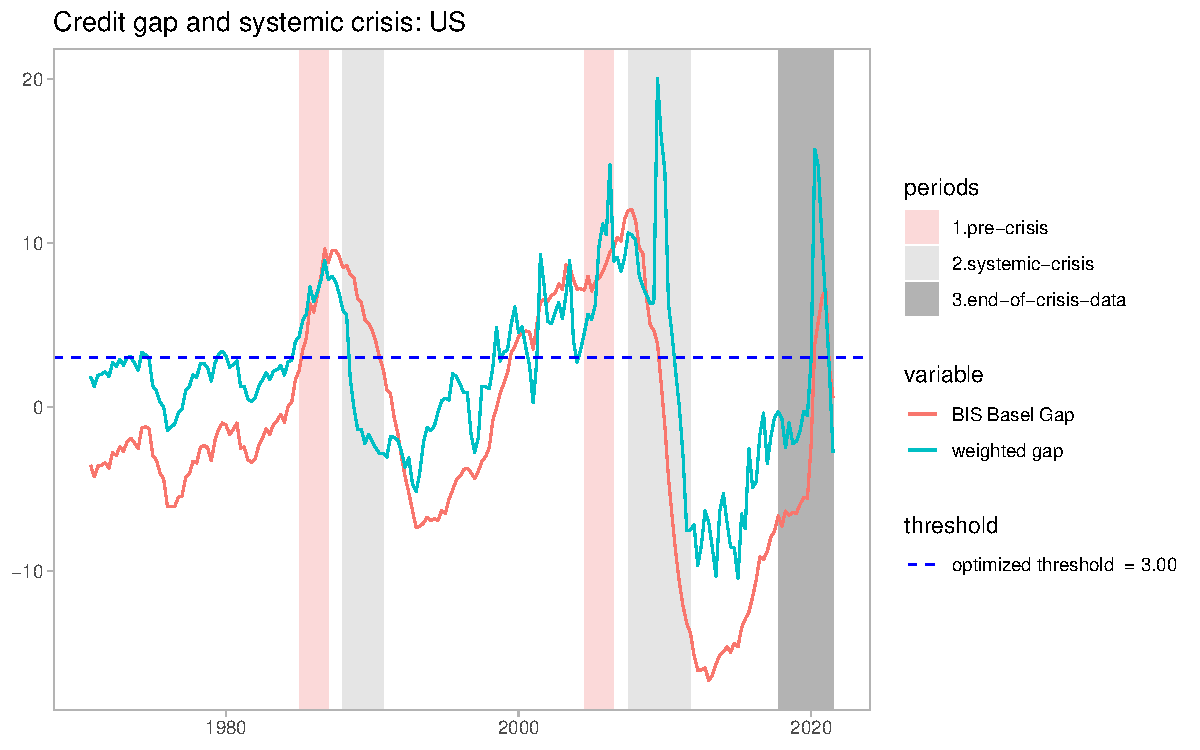
\includegraphics[width=1\linewidth]{../Data/Output/Graphs/Weighted_credit_gap_US} 

}

\caption{US time series graph}\label{fig:wUS}
\end{figure}

\begin{figure}

{\centering 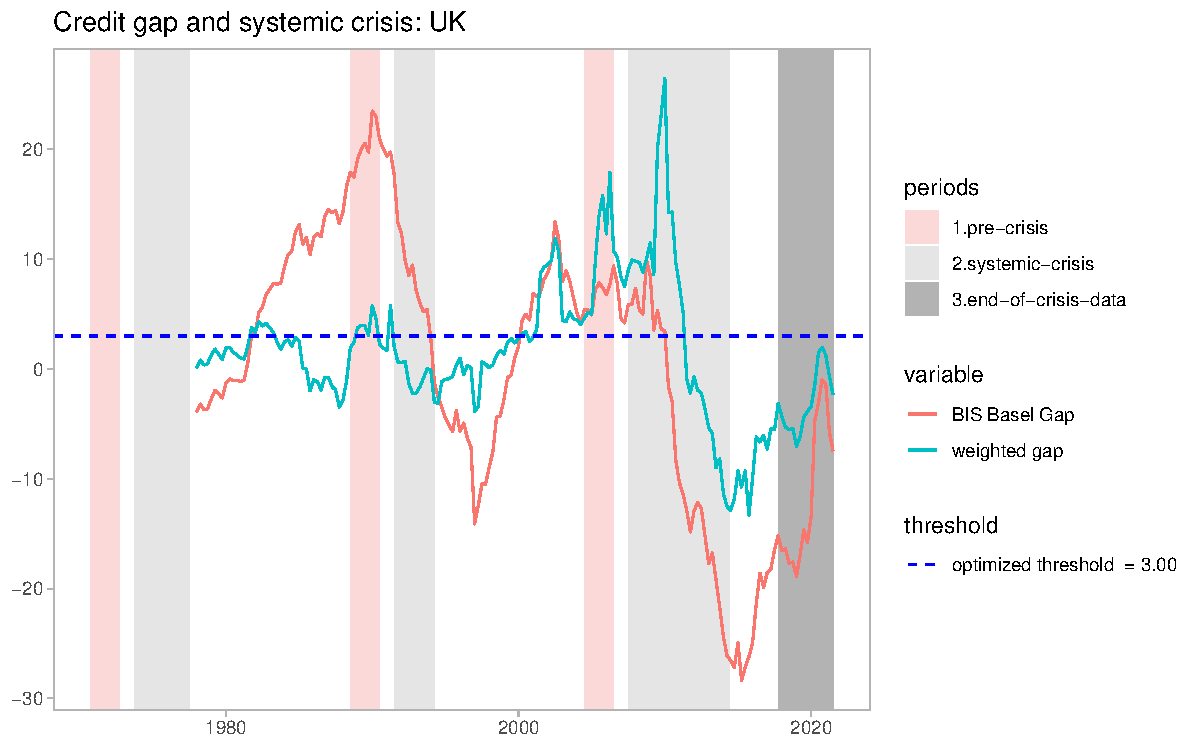
\includegraphics[width=1\linewidth]{../Data/Output/Graphs/Weighted_credit_gap_UK} 

}

\caption{UK time series graph}\label{fig:wUK}
\end{figure}

For the US, the weighted gap and BIS Basel gap performed similarly. They were able to predict the late 80s - early 90s financial crisis. They raised above the threshold starting early 2000s, which would result in misclassification of pre-crisis periods (Type I error) since our model wants to only identify periods of 5-12 months before a systemic financial crisis that would not happen until 2008. Nevertheless, the two gap series showed a build-up of an unsustainable credit gap for a prolonged period before the Great Financial Crisis (GFC) in the US. It is also worth pointing out that the weighted gap dipped below the threshold again before climbing again to identify the pre-crisis period of the GFC correctly.

The graph for the UK tells quite a similar story to the US. Both the credit gaps were able to detect the pre-crisis periods in the early 1990s and the GFC on 2008 for the UK. However, regarding the 90s crisis, the BIS Basel gap went above its threshold too early, for about five years. This could trigger unnecessary counter-cyclical buffer measurements from the central bank and cause the economy to slow its growth rate because of credit constraints. The weighted gap performed much better than the BIS Basel gap as it only sent out the signal during the pre-crisis period of the early 1990s for the UK.

From the graphical features of the weighted gap, we can compare the magnitude and length of the weighted gaps to that of the BIS Basel gap, which has long, smooth trends. Additionally, the weighted gap also retains the more volatile features and short spikes of sudden credit growth that the Beveridge-Nelson and other shorter-term cycle decomposition methods have. These averaged features help explain the averaged method's improved performance as an EWI over other traditional decomposition filters.

From here, to continue our analysis beyond 2017:Q4, we extrapolated our weights on one-sided credit gaps as constants to create a weighted credit gap outside of the crisis data range. This allows us to extrapolate our prediction until 2021:Q3. In response to COVID-19, most countries increased their total credit through multiple monetary policies, or their GDP growth slowed down, both of which created a significant upswing in the magnitude of the credit gap measurement above its optimized pre-crisis detection threshold. Per Drehmann \& Yetman (\protect\hyperlink{ref-drehmann_which_2021}{2021}), a good EWI signal would have the ideal characteristic of a stable signal meaning the credit gap need to be above the threshold and remain stable above the threshold during the pre-crisis period. We assume from our model finding that an economy with a credit gap above its optimized threshold for 8 consecutive quarters has a 2/3rd chance of having a financial crisis after the next 4 quarters.

As for the US, even though its credit gap was above the threshold for a few quarters, the gap eventually dropped below the threshold. This does not give us enough evidence to suggest that the country is at risk of a systemic financial crisis in the short future. However, there was an increase in the risk of crisis as the credit gap went beyond the threshold substantially during COVID-19 period. For the UK, the credit gaps did not exceed its threshold. Therefore, there is no evidence to show that the UK is at risk of a future financial crisis.

We performed a graphical analysis of all the countries in the sample and identified countries with significant credit gaps above the optimized 3.00 credit gap threshold beyond the 2017:Q4 crisis data limit window. We selected nine countries with signs of being at pre-crisi riskand should have performed pre-emptive macroprudential measures. They are Canada, France, Hong Kong (SAR), Japan, South Korea, Saudi Arabia, Switzerland, Sweden, and Thailand.\footnote{graphs of those countries are included in Appendix \ref{graphs-other}}

There are three outliers in those nine countries: Canada, Switzerland, and Hong Kong (SAR). Since the end of the GFC, the credit gaps in these three countries have been substantially above their optimized threshold. Additionally, those three countries never experienced systemic financial crises. Therefore, the EWI model performance for those three countries is not robust, and the evidence only comes from abroad. The other six countries: France, Switzerland, Japan, South Korea, Saudi Arabia, and Thailand, have evidence to show that pre-emptive macroprudential measures are to be performed to reduce the risk of having a systemic crisis.

\hypertarget{conclusion}{%
\section{Conclusion}\label{conclusion}}

Our study is based on the idea that excessive credit growth measured by the total credit to GDP deviations could be used as an early warning indicator for future systemic financial crises. We build a novel framework to select relevant credit gap decomposition filters, average their combinations, and create a crisis-weighted credit gap that inherits the combined features of the selected filters. We also proposed a novel performance metric for early warning indicator psAUC with a specific constraint that has appealing policy implication properties.

Our findings in this paper provide robust evidence to show the superior predictive performance of our proposed weighted credit gap over other univariate early warning indicator models that use individual credit gap filters. The novel proposed metric psAUC also showed that it has appealing properties for policy maker. It simplifies the steps to search for a decomposition filter with minimized loss function in the range of credit gap thresholds with Type II error rates smaller than 1/3. Therefore, the weighted gap and novel metric can be regarded as useful additional reference points for policy implications.

\clearpage

\hypertarget{references}{%
\section*{References}\label{references}}
\addcontentsline{toc}{section}{References}

\hypertarget{refs}{}
\begin{CSLReferences}{1}{0}
\leavevmode\vadjust pre{\hypertarget{ref-aldasoro_early_2018}{}}%
Aldasoro, I., Borio, C. E. V., \& Drehmann, M. (2018). \emph{\href{https://papers.ssrn.com/abstract=3139160}{Early {Warning Indicators} of {Banking Crises}: {Expanding} the {Family}}} (SSRN Scholarly Paper No. ID 3139160). {Rochester, NY}: {Social Science Research Network}.

\leavevmode\vadjust pre{\hypertarget{ref-alessi_identifying_2018}{}}%
Alessi, L., \& Detken, C. (2018). \href{https://doi.org/10.1016/j.jfs.2017.06.005}{Identifying excessive credit growth and leverage}. \emph{Journal of Financial Stability}, \emph{35}, 215--225.

\leavevmode\vadjust pre{\hypertarget{ref-babecky_banking_2014}{}}%
Babecký, J., Havránek, T., Matějů, J., Rusnák, M., Šmídková, K., \& Vašíček, B. (2014). \href{https://doi.org/10.1016/j.jfs.2014.07.001}{Banking, debt, and currency crises in developed countries: {Stylized} facts and early warning indicators}. \emph{Journal of Financial Stability}, \emph{15}, 1--17.

\leavevmode\vadjust pre{\hypertarget{ref-basel_guidance_2010}{}}%
Banking Supervision (2010), B. C. on. (2010). Guidance for national authorities operating the countercyclical capital buffer. \emph{Bank for International Settlements, December.}

\leavevmode\vadjust pre{\hypertarget{ref-beltran_optimizing_2021}{}}%
Beltran, D. O., Jahan-Parvar, M. R., \& Paine, F. A. (2021). \href{https://doi.org/10.17016/IFDP.2021.1307}{Optimizing {Credit Gaps} for {Predicting Financial Crises}: {Modelling Choices} and {Tradeoffs}}. \emph{International Finance Discussion Paper}, \emph{2021}, 1--40.

\leavevmode\vadjust pre{\hypertarget{ref-borio_financial_2014}{}}%
Borio, C. (2014). \href{https://doi.org/10.1016/j.jbankfin.2013.07.031}{The financial cycle and macroeconomics: {What} have we learnt?} \emph{Journal of Banking \& Finance}, \emph{45}, 182--198.

\leavevmode\vadjust pre{\hypertarget{ref-borio_assessing_2009}{}}%
Borio, C. E. V., \& Drehmann, M. (2009). \emph{\href{https://papers.ssrn.com/abstract=1513316}{Assessing the {Risk} of {Banking Crises} -- {Revisited}}} (SSRN Scholarly Paper No. ID 1513316). {Rochester, NY}: {Social Science Research Network}.

\leavevmode\vadjust pre{\hypertarget{ref-borio_assessing_2002}{}}%
Borio, C., \& Lowe, P. (2002). Assessing the risk of banking crises. \emph{BIS Quarterly Review}, \emph{7}, 43--54.

\leavevmode\vadjust pre{\hypertarget{ref-campagnoli_dynamic_2009}{}}%
Campagnoli, P., Petrone, S., \& Petris, G. (2009). \emph{\href{https://doi.org/10.1007/b135794}{Dynamic {Linear Models} with {R}}}. {New York, NY}: {Springer New York}.

\leavevmode\vadjust pre{\hypertarget{ref-carpenter_bootstrap_2000}{}}%
Carpenter, J., \& Bithell, J. (2000). \href{https://doi.org/10.1002/(SICI)1097-0258(20000515)19:9\%3C1141::AID-SIM479\%3E3.0.CO;2-F}{Bootstrap confidence intervals: When, which, what? {A} practical guide for medical statisticians}. \emph{Statistics in Medicine}, \emph{19}, 1141--1164.

\leavevmode\vadjust pre{\hypertarget{ref-detken_operationalising_2014}{}}%
Detken, C., Weeken, O., Alessi, L., Bonfim, D., Boucinha, M., Castro, C., \ldots{} Welz, P. (2014). Operationalising the {Countercyclical Capital Buffer}: {Indicator Selection}, {Threshold Identification} and {Calibration Options}. \emph{SSRN Electronic Journal}. \url{https://doi.org/10.2139/ssrn.3723336}

\leavevmode\vadjust pre{\hypertarget{ref-drehmann_evaluating_2014}{}}%
Drehmann, M., \& Juselius, M. (2014). \href{https://doi.org/10.1016/j.ijforecast.2013.10.002}{Evaluating early warning indicators of banking crises: {Satisfying} policy requirements}. \emph{International Journal of Forecasting}, \emph{30}, 759--780.

\leavevmode\vadjust pre{\hypertarget{ref-drehmann_credit_2014}{}}%
Drehmann, M., \& Tsatsaronis, K. (2014). \emph{\href{https://papers.ssrn.com/abstract=2457108}{The {Credit-to-GDP Gap} and {Countercyclical Capital Buffers}: {Questions} and {Answers}}} (SSRN Scholarly Paper No. ID 2457108). {Rochester, NY}: {Social Science Research Network}.

\leavevmode\vadjust pre{\hypertarget{ref-drehmann_why_2018}{}}%
Drehmann, M., \& Yetman, J. (2018). \emph{Why you should use the {Hodrick-Prescott} filter - at least to generate credit gaps}. 24.

\leavevmode\vadjust pre{\hypertarget{ref-drehmann_which_2021}{}}%
Drehmann, M., \& Yetman, J. (2021). Which {Credit Gap Is Better} at {Predicting Financial Crises}? {A Comparison} of {Univariate Filters}. \emph{International Journal of Central Banking}, 31.

\leavevmode\vadjust pre{\hypertarget{ref-furnival_regressions_2000}{}}%
Furnival, G. M., \& Wilson, R. W. (2000). Regressions by leaps and bounds. \emph{Technometrics}, \emph{42}, 69--79.

\leavevmode\vadjust pre{\hypertarget{ref-galan_measuring_2019}{}}%
Galán, J. (2019). Measuring {Credit-To-GDP Gaps}. {The Hodrick-Prescott Filter Revisited}. \emph{SSRN Electronic Journal}. \url{https://doi.org/10.2139/ssrn.3384613}

\leavevmode\vadjust pre{\hypertarget{ref-gerdrup_key_2013}{}}%
Gerdrup, K., Kvinlog, A. B., \& Schaanning, E. (2013). \emph{Key indicators for a countercyclical capital buffer in {Norway} - {Trends} and {Uncertainty}}. 44.

\leavevmode\vadjust pre{\hypertarget{ref-hamilton_why_2018}{}}%
Hamilton, J. D. (2018). \href{https://doi.org/10.1162/rest_a_00706}{Why {You Should Never Use} the {Hodrick-Prescott Filter}}. \emph{The Review of Economics and Statistics}, \emph{100}, 831--843.

\leavevmode\vadjust pre{\hypertarget{ref-holopainen_toward_2017}{}}%
Holopainen, M., \& Sarlin, P. (2017). \href{https://doi.org/10.1080/14697688.2017.1357972}{Toward robust early-warning models: A horse race, ensembles and model uncertainty}. \emph{Quantitative Finance}, \emph{17}, 1933--1963.

\leavevmode\vadjust pre{\hypertarget{ref-kaminsky_twin_1999}{}}%
Kaminsky, G. L., \& Reinhart, C. M. (1999). The {Twin Crises}: {The Causes} of {Banking} and {Balance-of-Payments Problems}. \emph{THE AMERICAN ECONOMIC REVIEW}, \emph{89}, 132.

\leavevmode\vadjust pre{\hypertarget{ref-madigan_bayesian_1995}{}}%
Madigan, D., York, J., \& Allard, D. (1995). \href{https://doi.org/10.2307/1403615}{Bayesian {Graphical Models} for {Discrete Data}}. \emph{International Statistical Review / Revue Internationale de Statistique}, \emph{63}, 215.

\leavevmode\vadjust pre{\hypertarget{ref-manias_panics_1978}{}}%
Manias, K. C. (1978). Panics, and crashes: {A} history of financial crises. \emph{Kindleberger---Basic Books.---1978.---272}.

\leavevmode\vadjust pre{\hypertarget{ref-mcclish_analyzing_1989}{}}%
McClish, D. K. (1989). \href{https://doi.org/10.1177/0272989X8900900307}{Analyzing a {Portion} of the {ROC Curve}}. \emph{Medical Decision Making}, \emph{9}, 190--195.

\leavevmode\vadjust pre{\hypertarget{ref-minsky_financial_1977}{}}%
Minsky, H. P. (1977). The financial instability hypothesis: {An} interpretation of {Keynes} and an alternative to {``standard''} theory. \emph{Challenge}, \emph{20}, 20--27.

\leavevmode\vadjust pre{\hypertarget{ref-raftery_bayesian_1995}{}}%
Raftery, A. E. (1995). \href{https://doi.org/10.2307/271063}{Bayesian {Model Selection} in {Social Research}}. \emph{Sociological Methodology}, \emph{25}, 111.

\leavevmode\vadjust pre{\hypertarget{ref-robin_proc_2011}{}}%
Robin, X., Turck, N., Hainard, A., Tiberti, N., Lisacek, F., Sanchez, J.-C., \& Müller, M. (2011). \href{https://doi.org/10.1186/1471-2105-12-77}{{pROC}: An open-source package for {R} and {S}+ to analyze and compare {ROC} curves}. \emph{BMC Bioinformatics}, \emph{12}, 77.

\end{CSLReferences}

\hypertarget{appendix-appendix}{%
\appendix}


\hypertarget{appendix}{%
\section{Appendix}\label{appendix}}

\hypertarget{filterslist}{%
\subsection{List of complete decomposition filters used in the model selection process}\label{filterslist}}

All filters are in (quasi-real time) one-sided fashion. We store the value of the decomposed cycles for the current period permanently as data becomes available and will not change it when new data comes in the next period.

\textbf{Hodrick Prescott (HP) filters with different smoothing parameters \(\lambda\):\\
}- c.hp, c.hp3k, c.hp25k, c.hp125k, c.hp221k, c.hp400k

\textbf{Hamilton filters with different smoothing parameters \(\theta\) (distance of past lags):\\
}- c.hamilton13, c.hamilton20, c.hamilton24, c.hamilton28

\textbf{Linear and polynomial filter models:\\
}- c.linear, c.quad, c.poly3, c.poly4, c.poly5, c.poly6

\textbf{Beveridge-Nelson decomposition filters with different smoothing parameters (number of lags):\\
}- c.bn2, c.bn3, c.bn4, c.bn5, c.bn6, c.bn7, c.bn8

\textbf{Structural time series model:\\
}- c.stm

\textbf{Rolling sample with 15 and 20 years window (of all previous filters in 1-5 ):\\
}- c.hp\_r15, c.hp3k\_r15, c.hp25k\_r15, c.hp125k\_r15, c.hp221k\_r15, c.hp400k\_r15, c.hamilton13\_r15, c.hamilton20\_r15, c.hamilton24\_r15, c.hamilton28\_r15, c.linear\_r15, c.quad\_r15, c.poly3\_r15, c.poly4\_r15, c.poly5\_r15, c.poly6\_r15, c.bn2\_r15, c.bn3\_r15, c.bn4\_r15, c.bn5\_r15, c.bn6\_r15, c.bn7\_r15, c.bn8\_r15, c.stm\_r15
- c.hp\_r20, c.hp3k\_r20, c.hp25k\_r20, c.hp125k\_r20, c.hp221k\_r20, c.hp400k\_r20, c.hamilton13\_r20, c.hamilton20\_r20, c.hamilton24\_r20, c.hamilton28\_r20, c.linear\_r20, c.quad\_r20, c.poly3\_r20, c.poly4\_r20, c.poly5\_r20, c.poly6\_r20, c.bn2\_r20, c.bn3\_r20, c.bn4\_r20, c.bn5\_r20, c.bn6\_r20, c.bn7\_r20, c.bn8\_r20, c.stm\_r20

\textbf{Hamilton filters in panel setting (with rolling samples):\\
}- c.hamilton13\_panel, c.hamilton20\_panel, c.hamilton24\_panel, c.hamilton28\_panel, c.hamilton13\_panelr15, c.hamilton20\_panelr15, c.hamilton24\_panelr15, c.hamilton28\_panelr15, c.hamilton13\_panelr20, c.hamilton20\_panelr20, c.hamilton24\_panelr20, c.hamilton28\_panelr20

\textbf{Moving Average filter:\\
}- c.ma

All models are given equal prior weights.

\hypertarget{ma-stm-eq}{%
\subsection{Statistical Methods for Trend-Cycle Decomposition}\label{ma-stm-eq}}

\hypertarget{bayesian-structural-time-series-model-stm}{%
\subsubsection*{Bayesian structural time series model (STM)}\label{bayesian-structural-time-series-model-stm}}
\addcontentsline{toc}{subsubsection}{Bayesian structural time series model (STM)}

\begin{align*}
y_t = u_t + v_t,  vt \sim N(0,V)\\
u_t = u_{t-1} + \beta_{t-1} + w_{1,t},  w_{1,t} \sim N(O,\sigma^2_{w1})\\
\beta_t = \beta_{t_1} + w_{2,t},  w_{2,t} \sim N(0,\sigma^2_{w2})
\end{align*}

The implementation of this filter is discussed in (\protect\hyperlink{ref-campagnoli_dynamic_2009}{Campagnoli, Petrone, \& Petris, 2009}). One feature of this filter that allows for smoother trend component is its inclusion of a time-varying local growth rate \(\beta_t\). Beltran et al. (\protect\hyperlink{ref-beltran_optimizing_2021}{2021}) estimated the optimized the value of the smoothing parameter at \(\sigma^2_{w1} = 1\) , \(\sigma^2_{w2}=0.01\) and V = 1100.

\hypertarget{moving-average}{%
\subsubsection*{Moving Average}\label{moving-average}}
\addcontentsline{toc}{subsubsection}{Moving Average}

\begin{align*}
MA_t = y_t - \frac{\sum\nolimits^t_{i=t-q+1}y_i}{q}
\end{align*}

With q being the smoothing parameter and the length of the moving average window. Beltran et al. (\protect\hyperlink{ref-beltran_optimizing_2021}{2021}) estimated the optimized value for parameter q to be 16.

\hypertarget{out-of-sample-forecast-graphs}{%
\subsection{Out of sample forecast graphs}\label{out-of-sample-forecast-graphs}}

\hypertarget{graphs-other}{%
\subsubsection{Graphs of selected countries}\label{graphs-other}}

\begin{figure}[H]

{\centering 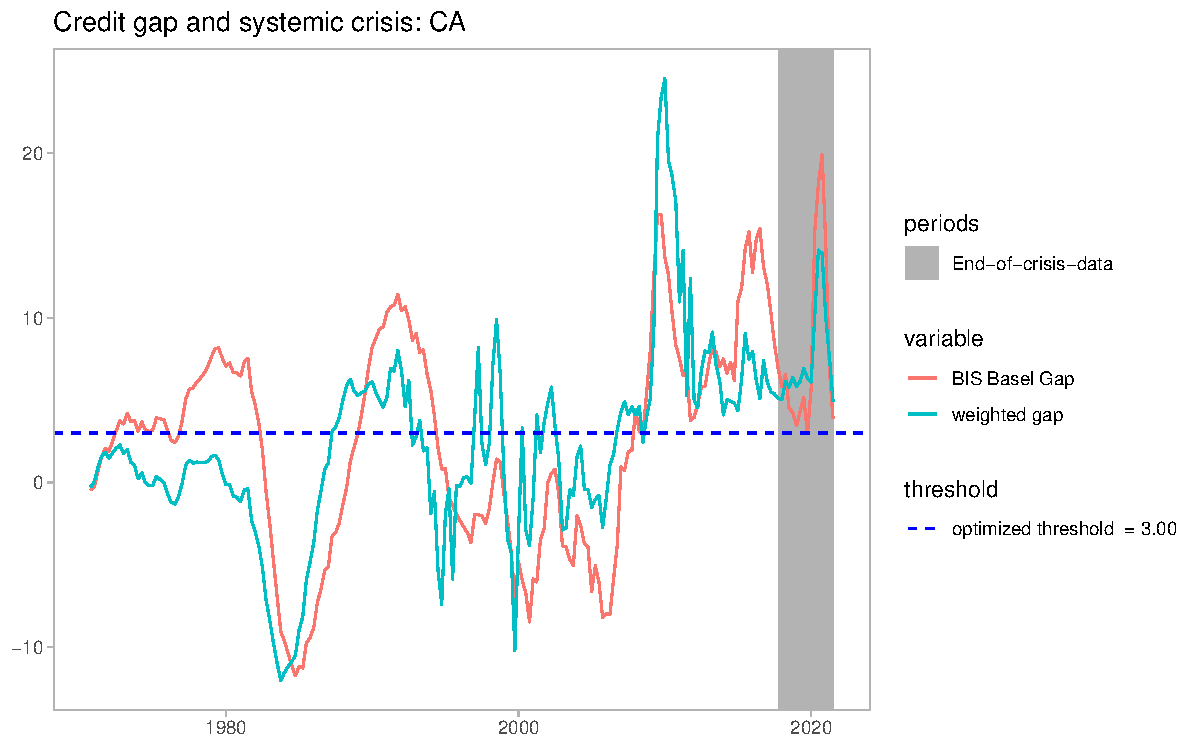
\includegraphics[width=0.85\linewidth]{../Data/Output/Graphs/All/Weighted_credit_gap_CA} 

}

\caption{Canada time series graph}\label{fig:CAseries}
\end{figure}

\begin{figure}[H]

{\centering 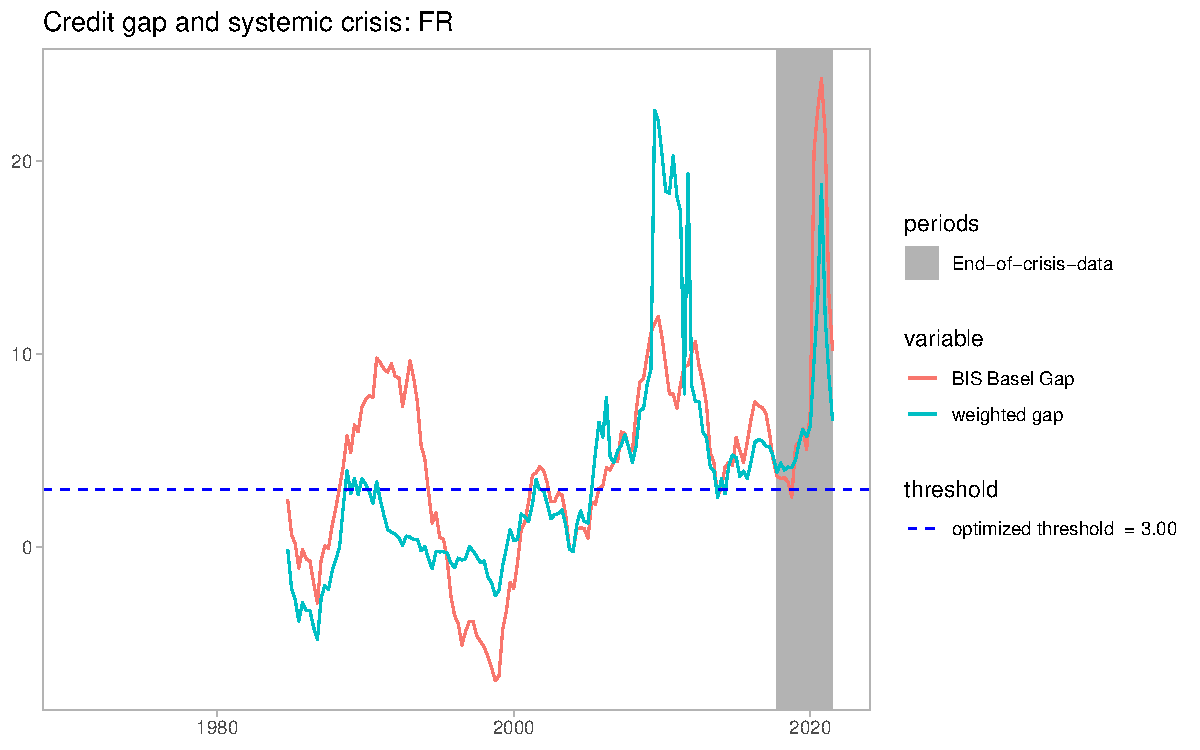
\includegraphics[width=0.85\linewidth]{../Data/Output/Graphs/All/Weighted_credit_gap_FR} 

}

\caption{France time series graph}\label{fig:FRseries}
\end{figure}

\begin{figure}[H]

{\centering 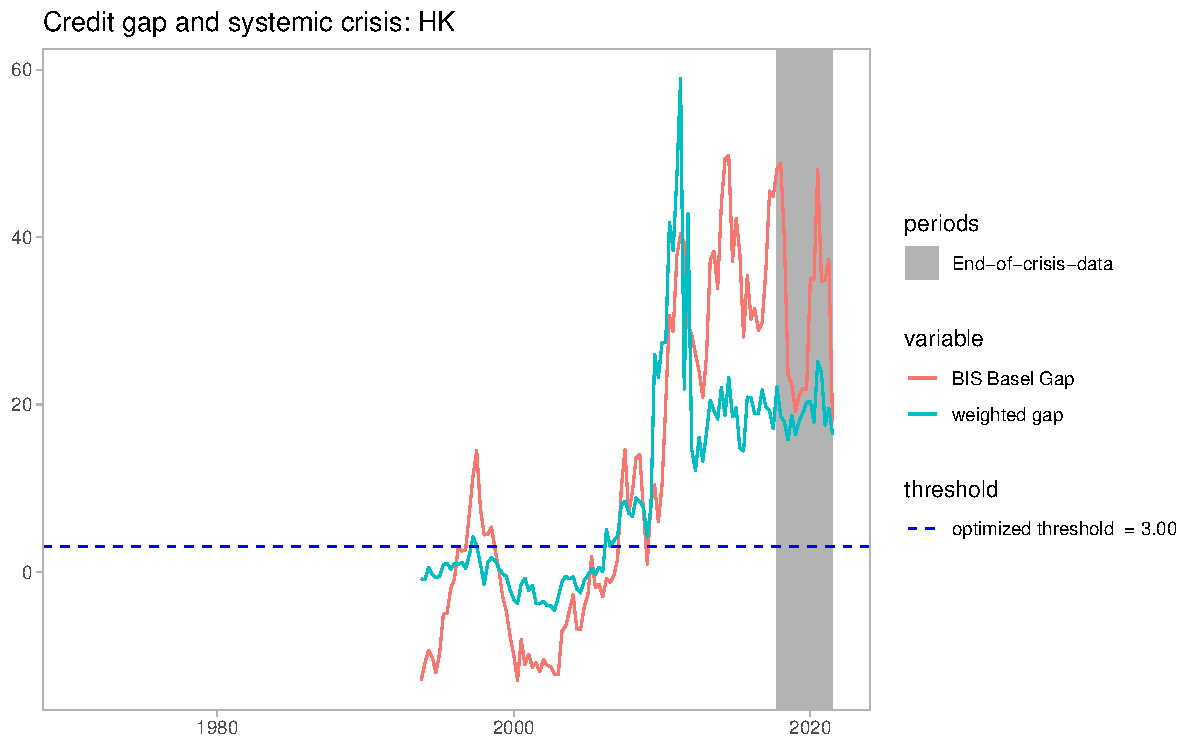
\includegraphics[width=0.85\linewidth]{../Data/Output/Graphs/All/Weighted_credit_gap_HK} 

}

\caption{Hong Kong time series graph}\label{fig:HKseries}
\end{figure}

\begin{figure}[H]

{\centering 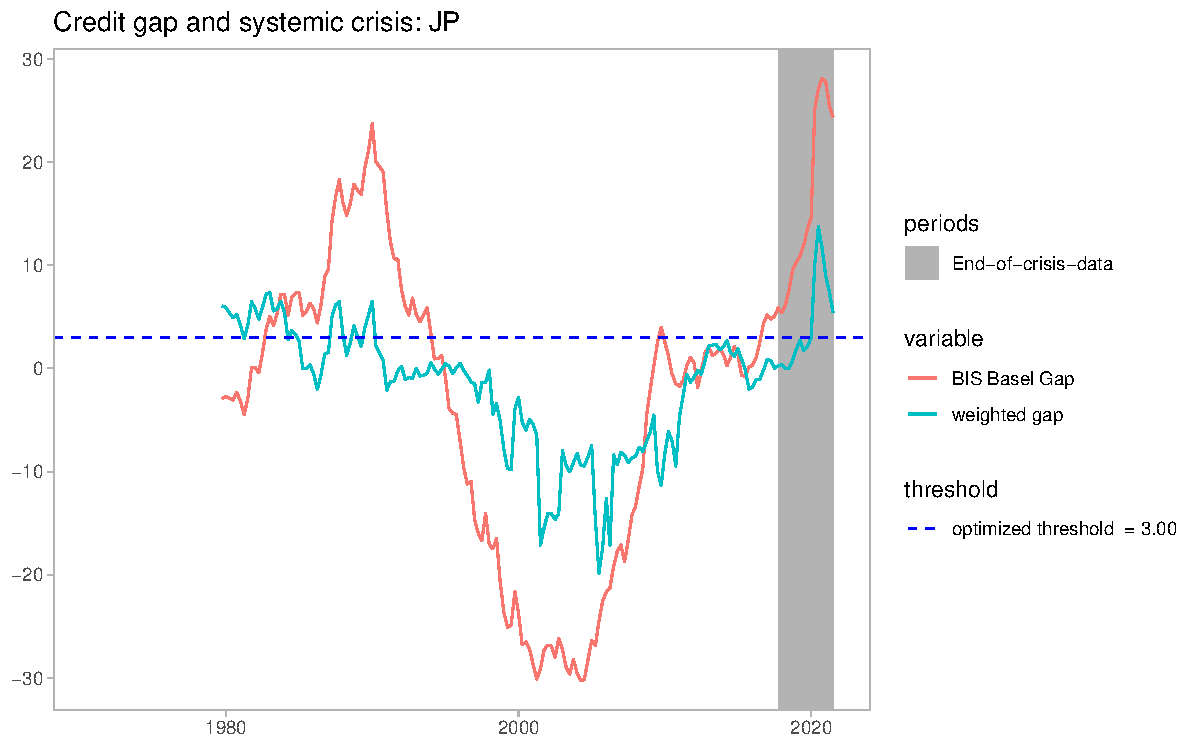
\includegraphics[width=0.85\linewidth]{../Data/Output/Graphs/All/Weighted_credit_gap_JP} 

}

\caption{Japan time series graph}\label{fig:JPseries}
\end{figure}

\begin{figure}[H]

{\centering 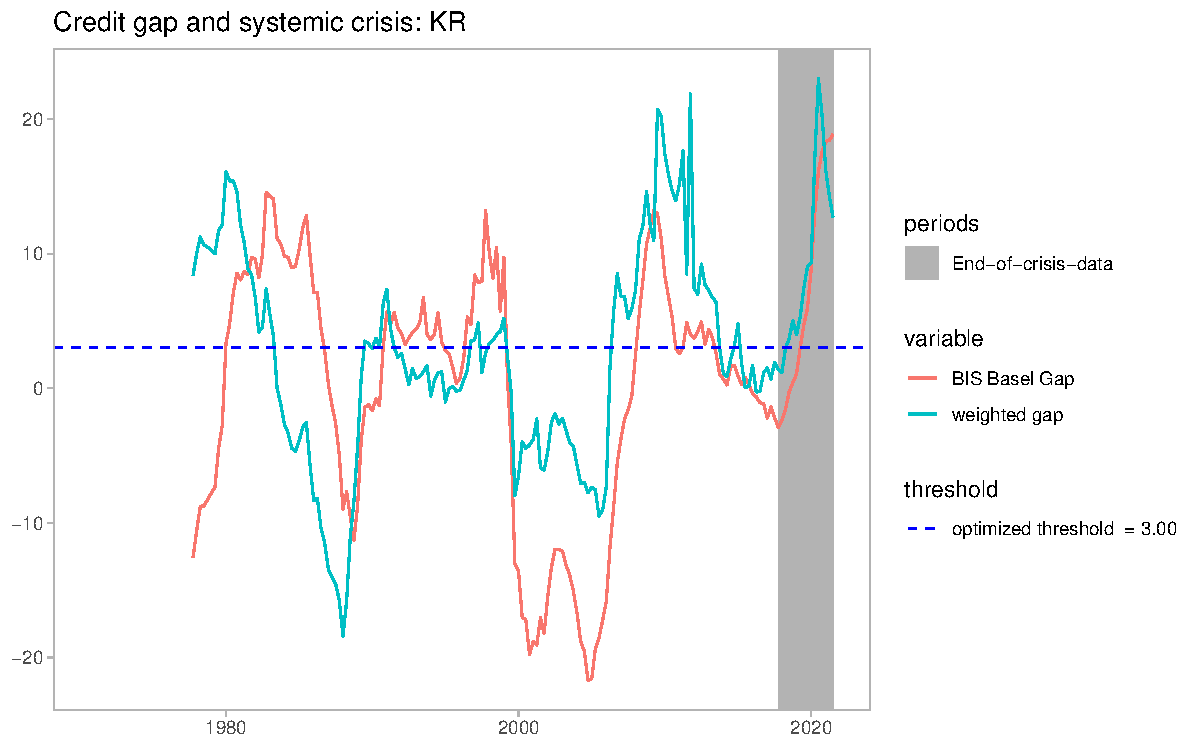
\includegraphics[width=0.85\linewidth]{../Data/Output/Graphs/All/Weighted_credit_gap_KR} 

}

\caption{South Korea time series graph}\label{fig:KRseries}
\end{figure}

\begin{figure}[H]

{\centering 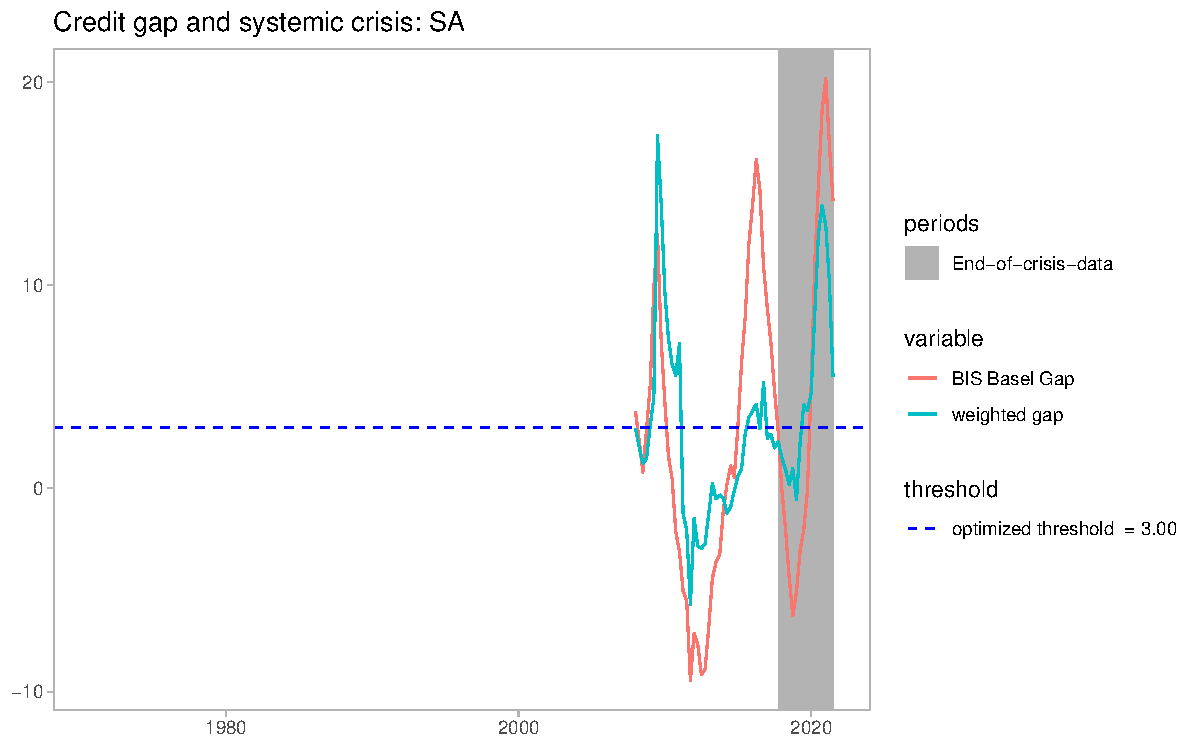
\includegraphics[width=0.85\linewidth]{../Data/Output/Graphs/All/Weighted_credit_gap_SA} 

}

\caption{Saudi Arabia time series graph}\label{fig:SAseries}
\end{figure}

\begin{figure}[H]

{\centering 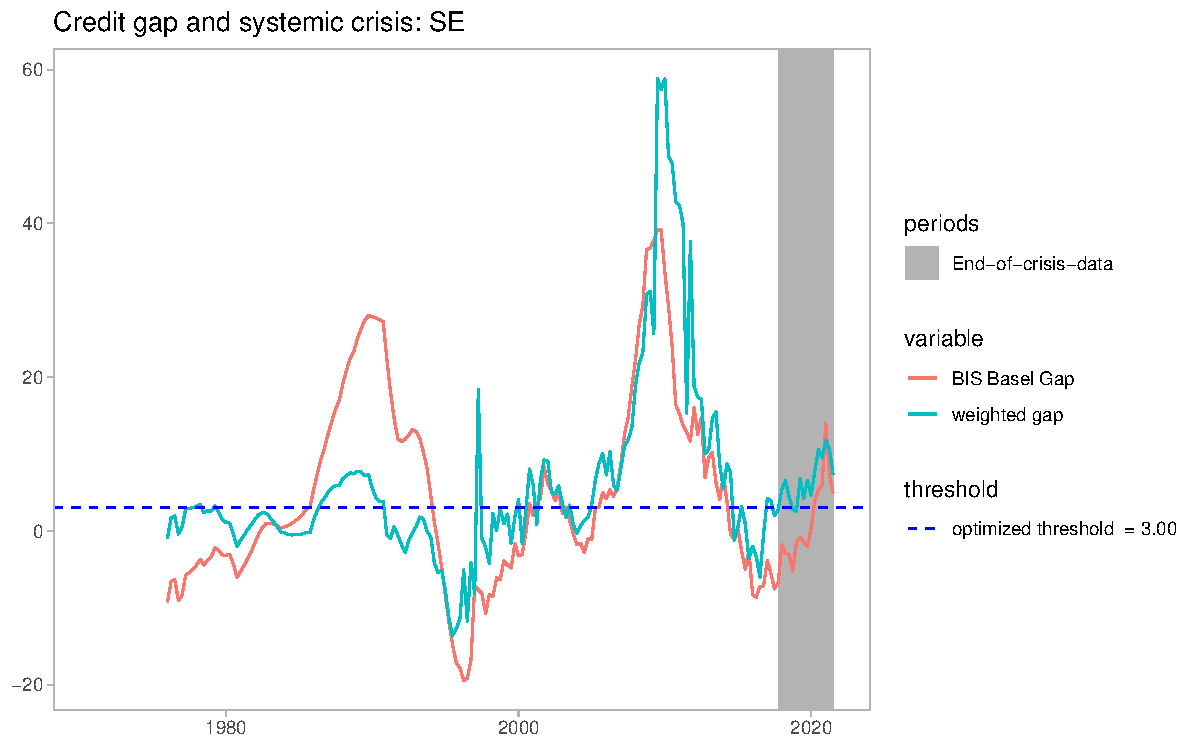
\includegraphics[width=0.85\linewidth]{../Data/Output/Graphs/All/Weighted_credit_gap_SE} 

}

\caption{Sweden time series graph}\label{fig:SEseries}
\end{figure}

\begin{figure}[H]

{\centering 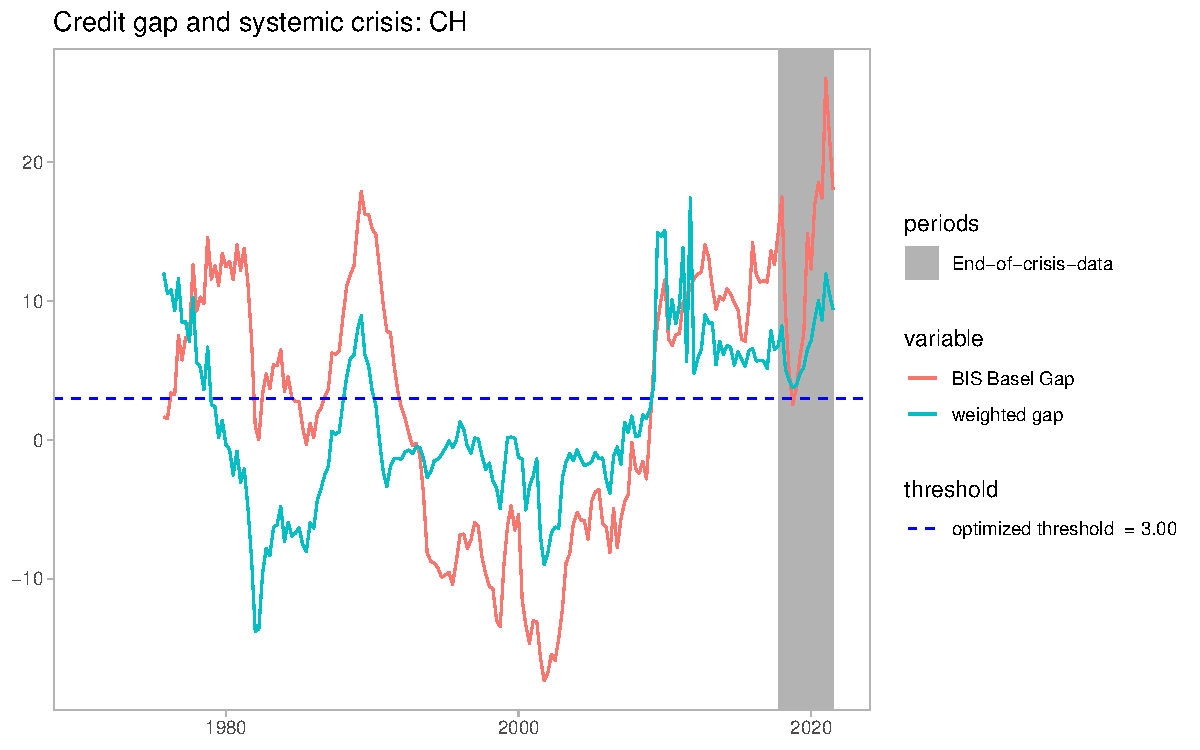
\includegraphics[width=0.85\linewidth]{../Data/Output/Graphs/All/Weighted_credit_gap_CH} 

}

\caption{Switzerland time series graph}\label{fig:CHseries}
\end{figure}

\begin{figure}[H]

{\centering 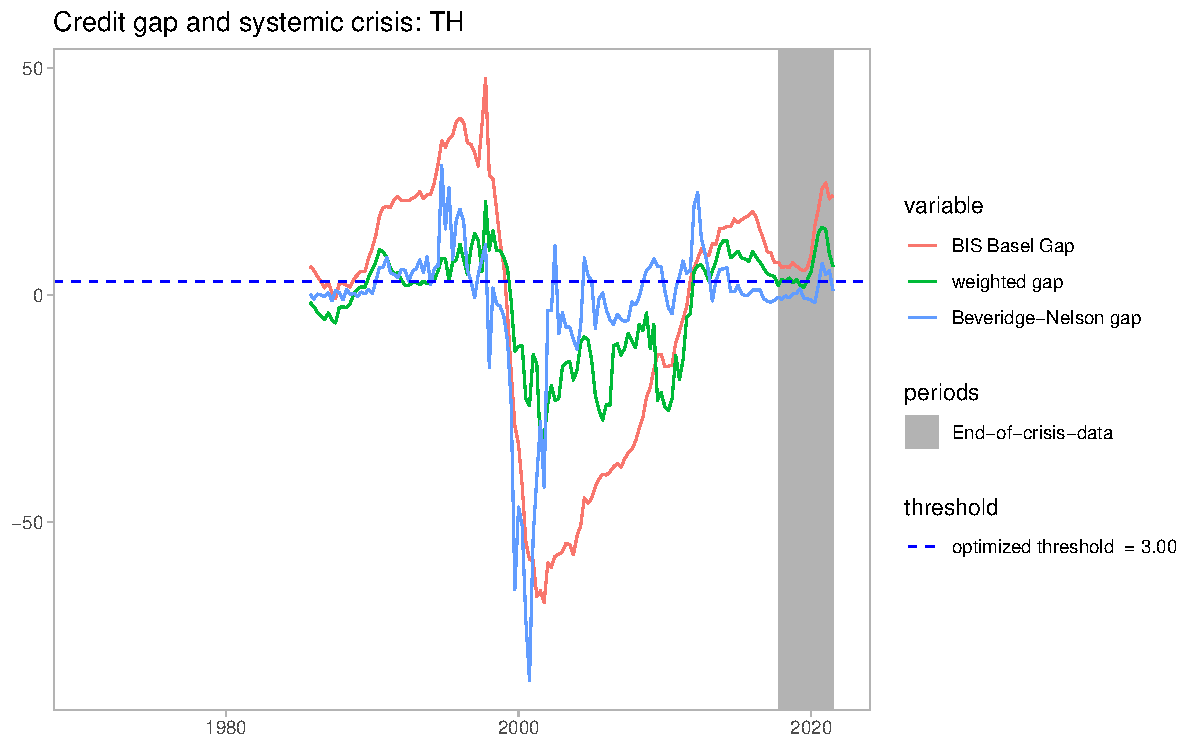
\includegraphics[width=0.85\linewidth]{../Data/Output/Graphs/All/Weighted_credit_gap_TH} 

}

\caption{Thailand time series graph}\label{fig:THseries}
\end{figure}

\end{document}
